\documentclass[10pt,fleqn]{article} % Default font size and left-justified equations
\usepackage[%
    pdftitle={RdM : Diagrammes de sollicitations},
    pdfauthor={Xavier Pessoles}]{hyperref}
    
%%%%%%%%%%%%%%%%%%%%%%%%%%%%%%%%%%%%%%%%%
% Original author:
% Mathias Legrand (legrand.mathias@gmail.com) with modifications by:
% Vel (vel@latextemplates.com)
% License:
% CC BY-NC-SA 3.0 (http://creativecommons.org/licenses/by-nc-sa/3.0/)
%%%%%%%%%%%%%%%%%%%%%%%%%%%%%%%%%%%%%%%%%

%----------------------------------------------------------------------------------------
%	VARIOUS REQUIRED PACKAGES AND CONFIGURATIONS
%----------------------------------------------------------------------------------------

\usepackage[top=2.5cm,bottom=2cm,left=2cm,right=2cm,headsep=40pt,a4paper]{geometry} % Page margins

\usepackage{graphicx} % Required for including pictures
\graphicspath{{images/}} % Specifies the directory where pictures are stored

\usepackage{lipsum} % Inserts dummy text

\usepackage{tikz} % Required for drawing custom shapes

\usepackage[french]{babel} % English language/hyphenation
\frenchbsetup{StandardLists=true} % Pour éviter la collision babel enumitem pour les listes

\usepackage{enumitem} % Customize lists
\setlist{nolistsep} % Reduce spacing between bullet points and numbered lists

\usepackage{booktabs} % Required for nicer horizontal rules in tables

\usepackage{xcolor} % Required for specifying colors by name
%\definecolor{ocre}{RGB}{243,102,25} % Define the orange color used for highlighting throughout the book
 \definecolor{ocre}{RGB}{49,133,156} % Couleur ''bleue''
\definecolor{violetf}{RGB}{112,48,160} % Couleur ''violet''
\usepackage{enumitem}
\usepackage{pifont} % Pour les dinglist
\usepackage{multicol}
\usepackage{array} % Centrage vertical dans les tableaux

%----------------------------------------------------------------------------------------
%	FONTS
%----------------------------------------------------------------------------------------

\usepackage{avant} % Use the Avantgarde font for headings
%\usepackage{times} % Use the Times font for headings
%\usepackage{mathptmx} % Use the Adobe Times Roman as the default text font together with math symbols from the Sym­bol, Chancery and Com­puter Modern fonts
\usepackage[adobe-utopia]{mathdesign}
\usepackage{microtype} % Slightly tweak font spacing for aesthetics
\usepackage[utf8]{inputenc} % Required for including letters with accents
\usepackage[T1]{fontenc} % Use 8-bit encoding that has 256 glyphs

%----------------------------------------------------------------------------------------
%	BIBLIOGRAPHY AND INDEX
%----------------------------------------------------------------------------------------

\usepackage[style=alphabetic,citestyle=numeric,sorting=nyt,sortcites=true,autopunct=true,babel=hyphen,hyperref=true,abbreviate=false,backref=true,backend=biber]{biblatex}
\addbibresource{bibliography.bib} % BibTeX bibliography file
\defbibheading{bibempty}{}

\usepackage{calc} % For simpler calculation - used for spacing the index letter headings correctly
\usepackage{makeidx} % Required to make an index
\makeindex % Tells LaTeX to create the files required for indexing

%----------------------------------------------------------------------------------------
%	MAIN TABLE OF CONTENTS
%----------------------------------------------------------------------------------------

\usepackage{titletoc} % Required for manipulating the table of contents

\setcounter{tocdepth}{2}     % Dans la table des matieres
\setcounter{secnumdepth}{2}

\contentsmargin{0cm} % Removes the default margin

% Part text styling
\titlecontents{part}[0cm]
{\addvspace{20pt}\centering\large\bfseries}
{}
{}
{}

% Chapter text styling
\titlecontents{chapter}[1.25cm] % Indentation
{\addvspace{12pt}\large\sffamily\bfseries} % Spacing and font options for chapters
{\color{ocre!60}\contentslabel[\Large\thecontentslabel]{1.25cm}\color{ocre}} % Chapter number
{\color{ocre}}  
{\color{ocre!60}\normalsize\;\titlerule*[.5pc]{.}\;\thecontentspage} % Page number

% Section text styling
\titlecontents{section}[1.25cm] % Indentation
{\addvspace{3pt}\sffamily\bfseries} % Spacing and font options for sections
{\color{ocre!60}\contentslabel[\thecontentslabel]{1.25cm} \color{ocre}} % Section number
{\color{ocre}}
{\hfill\color{ocre!60}\thecontentspage} % Page number
[]

% Subsection text styling
\titlecontents{subsection}[1.25cm] % Indentation
{\addvspace{1pt}\sffamily\small} % Spacing and font options for subsections
{\contentslabel[\thecontentslabel]{1.25cm}} % Subsection number
{}
{\ \titlerule*[.5pc]{.}\;\thecontentspage} % Page number
[]


% Subsection text styling
\titlecontents{subsubsection}[1.25cm] % Indentation
{\addvspace{1pt}\sffamily\small} % Spacing and font options for subsections
{\contentslabel[\thecontentslabel]{1.25cm}} % Subsection number
{}
{\ \titlerule*[.5pc]{.}\;\thecontentspage} % Page number
[]

% List of figures
\titlecontents{figure}[0em]
{\addvspace{-5pt}\sffamily}
{\thecontentslabel\hspace*{1em}}
{}
{\ \titlerule*[.5pc]{.}\;\thecontentspage}
[]

% List of tables
\titlecontents{table}[0em]
{\addvspace{-5pt}\sffamily}
{\thecontentslabel\hspace*{1em}}
{}
{\ \titlerule*[.5pc]{.}\;\thecontentspage}
[]

%----------------------------------------------------------------------------------------
%	MINI TABLE OF CONTENTS IN PART HEADS
%----------------------------------------------------------------------------------------

% Chapter text styling
\titlecontents{lchapter}[0em] % Indenting
{\addvspace{15pt}\large\sffamily\bfseries} % Spacing and font options for chapters
{\color{ocre}\contentslabel[\Large\thecontentslabel]{1.25cm}\color{ocre}} % Chapter number
{}  
{\color{ocre}\normalsize\sffamily\bfseries\;\titlerule*[.5pc]{.}\;\thecontentspage} % Page number

% Section text styling
\titlecontents{lsection}[0em] % Indenting
{\sffamily\small} % Spacing and font options for sections
{\contentslabel[\thecontentslabel]{1.25cm}} % Section number
{}
{}

% Subsection text styling
\titlecontents{lsubsection}[.5em] % Indentation
{\normalfont\footnotesize\sffamily} % Font settings
{}
{}
{}

%----------------------------------------------------------------------------------------
%	PAGE HEADERS
%----------------------------------------------------------------------------------------

\usepackage{fancyhdr} % Required for header and footer configuration



\pagestyle{fancy}
 \renewcommand{\headrulewidth}{0pt}
 \fancyhead{}
 \fancyhead[L]{%
 \noindent\begin{minipage}[c]{2.6cm}%
 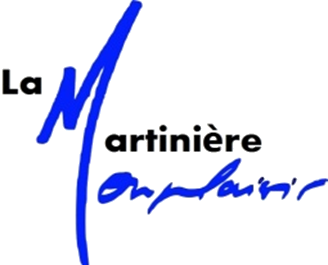
\includegraphics[width=2cm]{png/logo_lycee.png}%
 \end{minipage}}

\fancyhead[C]{\rule{8cm}{.5pt}}

 \fancyhead[R]{%
 \noindent\begin{minipage}[c]{3cm}
 \begin{flushright}
 \footnotesize{\textit{\textsf{\xxtete}}}%
 \end{flushright}
 \end{minipage}
}


\fancyfoot[C]{\rule{12cm}{.5pt}}
\renewcommand{\footrulewidth}{0.2pt}
\fancyfoot[C]{\footnotesize{\bfseries \thepage}}
\fancyfoot[L]{ 
\begin{minipage}[c]{.4\linewidth}
\noindent\footnotesize{{\xxauteur}}
\end{minipage}}


\fancyfoot[R]{\footnotesize{\xxpied}
\ifthenelse{\isodd{\value{page}}}{
\begin{tikzpicture}[overlay]
\node[shape=rectangle, 
      rounded corners = .25 cm,
	  draw= ocre,
	  line width=2pt, 
	  fill = ocre!10,
	  minimum width  = 2.5cm,
	  minimum height = 3cm,] at (\xxposongletx,\xxposonglety) {};
\node at (\xxposonglettext,\xxposonglety) {\rotatebox{90}{\textbf{\large\color{ocre}{\xxonglet}}}};
%{};
\end{tikzpicture}}{}
}
%
%
%
% Removes the header from odd empty pages at the end of chapters
\makeatletter
\renewcommand{\cleardoublepage}{
\clearpage\ifodd\c@page\else
\hbox{}
\vspace*{\fill}
\thispagestyle{empty}
\newpage
\fi}

\fancypagestyle{plain}{%
\fancyhf{} % vide l’en-tête et le pied~de~page.
%\fancyfoot[C]{\bfseries \thepage} % numéro de la page en cours en gras
% et centré en pied~de~page.
\fancyfoot[R]{\footnotesize{\xxpied}}
\fancyfoot[C]{\rule{12cm}{.5pt}}
\renewcommand{\footrulewidth}{0.2pt}
\fancyfoot[C]{\footnotesize{\bfseries \thepage}}
\fancyfoot[L]{ 
\begin{minipage}[c]{.4\linewidth}
\noindent\footnotesize{{\xxauteur}}
\end{minipage}}}



%----------------------------------------------------------------------------------------
%	THEOREM STYLES
%----------------------------------------------------------------------------------------

% Conflit avec la police adobe
%\usepackage{amsmath,amsfonts,amssymb,amsthm} % For math equations, theorems, symbols, etc
\usepackage{amsmath,amsthm}

\newcommand{\intoo}[2]{\mathopen{]}#1\,;#2\mathclose{[}}
\newcommand{\ud}{\mathop{\mathrm{{}d}}\mathopen{}}
\newcommand{\intff}[2]{\mathopen{[}#1\,;#2\mathclose{]}}
%\newtheorem{notation}{Notation}[chapter]
\newtheorem{notation}{Notation}[section]

% Boxed/framed environments
\newtheoremstyle{ocrenumbox}% % Theorem style name
{0pt}% Space above
{0pt}% Space below
{\normalfont}% % Body font
{}% Indent amount
{\small\bf\sffamily\color{ocre}}% % Theorem head font
{\;}% Punctuation after theorem head
{0.25em}% Space after theorem head
{\small\sffamily\color{ocre}\thmname{#1}\nobreakspace\thmnumber%{\@ifnotempty{#1}{}\@upn{#2}}% Theorem text (e.g. Theorem 2.1)
\thmnote{\nobreakspace\the\thm@notefont\sffamily\bfseries\color{black}---\nobreakspace#3.}} % Optional theorem note
\renewcommand{\qedsymbol}{$\blacksquare$}% Optional qed square


% Boite pour les corriges
\newtheoremstyle{correctionbox}% % Theorem style name
{0pt}% Space above
{0pt}% Space below
{\normalfont}% % Body font
{}% Indent amount
{\small\bf\sffamily\color{violet}}% % Theorem head font
{\;}% Punctuation after theorem head
{0.25em}% Space after theorem head
{\small\sffamily\color{ocre}\thmname{#1}\nobreakspace\thmnumber%{\@ifnotempty{#1}{}\@upn{#2}}% Theorem text (e.g. Theorem 2.1)
\thmnote{\nobreakspace\the\thm@notefont\sffamily\bfseries\color{black}---\nobreakspace#3.}} % Optional theorem note
\renewcommand{\qedsymbol}{$\blacksquare$}% Optional qed square



\newtheoremstyle{blacknumex}% Theorem style name
{5pt}% Space above
{5pt}% Space below
{\normalfont}% Body font
{} % Indent amount
{\small\bf\sffamily}% Theorem head font
{\;}% Punctuation after theorem head
{0.25em}% Space after theorem head
{\small\sffamily{\tiny\ensuremath{\blacksquare}}\nobreakspace\thmname{#1}\nobreakspace\thmnumber%{\@ifnotempty{#1}{}\@upn{#2}}% Theorem text (e.g. Theorem 2.1)
\thmnote{\nobreakspace\the\thm@notefont\sffamily\bfseries---\nobreakspace#3.}}% Optional theorem note

\newtheoremstyle{blacknumbox} % Theorem style name
{0pt}% Space above
{0pt}% Space below
{\normalfont}% Body font
{}% Indent amount
{\small\bf\sffamily}% Theorem head font
{\;}% Punctuation after theorem head
{0.25em}% Space after theorem head
{\small\sffamily\thmname{#1}\nobreakspace 
\thmnote{\nobreakspace\the\thm@notefont\sffamily\bfseries---\nobreakspace#3.}}% Optional theorem note

% Non-boxed/non-framed environments
\newtheoremstyle{ocrenum}% % Theorem style name
{5pt}% Space above
{5pt}% Space below
{\normalfont}% % Body font
{}% Indent amount
{\small\bf\sffamily\color{ocre}}% % Theorem head font
{\;}% Punctuation after theorem head
{0.25em}% Space after theorem head
{\small\sffamily\color{ocre}\thmname{#1}\nobreakspace%\thmnumber{\@ifnotempty{#1}{}\@upn{#2}}% Theorem text (e.g. Theorem 2.1)
\thmnote{\nobreakspace\the\thm@notefont\sffamily\bfseries\color{black}---\nobreakspace#3.}} % Optional theorem note
\renewcommand{\qedsymbol}{$\blacksquare$}% Optional qed square
\makeatother

% Environnement pour les titres de parties
\newtheoremstyle{partiebox} 
{0pt}% Space above
{0pt}% Space below
{\normalfont}% Body font
{}% Indent amount
{\small\bf\sffamily}% Theorem head font
{\;}% Punctuation after theorem head
{0.25em}% Space after theorem head




% Defines the theorem text style for each type of theorem to one of the three styles above
\newcounter{dummy} 
\numberwithin{dummy}{section}
\theoremstyle{ocrenumbox}
%\newtheorem{theoremeT}[dummy]{Théorème}
\newtheorem{theoremeT}[dummy]{Théorème}
\newtheorem{resultatT}[dummy]{Résultat}
\newtheorem{savoirT}[dummy]{Savoir}
\newtheorem{methodeT}[dummy]{Méthode}
\newtheorem{objectifT}[dummy]{Objectif}
%\newtheorem{problem}{Problem}[chapter]
\newtheorem{problem}{Problem}[section]
%\newtheorem{exerciseT}{Exercise}[chapter]
\newtheorem{exerciseT}{Exercice}[section]

\theoremstyle{blacknumex}
%\newtheorem{exampleT}{Example}[chapter]
\newtheorem{exempleT}{Exemple}[section]
\newtheorem{termT}{Terminal\\}[section]
\newtheorem{pyT}{Python\\}[section]
\newtheorem{sciT}{Scilab\\}[section]
\newtheorem{pseudoT}{Pseudo Code\\}[section]
\newtheorem{sqlT}{SQL\\}[section]

\theoremstyle{blacknumbox}
%\newtheorem{vocabulary}{Vocabulary}[chapter]
\newtheorem{vocabulary}{Vocabulaire}[section]
%\newtheorem{definitionT}{Definition}[section]
\newtheorem{definitionT}{Définition}[section]
\newtheorem{rappelT}{Rappel}[section]
\newtheorem{demoT}{Démonstration}[section]
\newtheorem{corollaryT}[dummy]{Corollaire}
\newtheorem{hypoT}{Hypothèse(s)}

\theoremstyle{ocrenum}
\newtheorem{proposition}[dummy]{Proposition}

\theoremstyle{partiebox}
\newtheorem{titrepartieT}[]{}
\newtheorem{titrechapitreT}[]{}

\theoremstyle{correctionbox}
\newtheorem{correctionT}[dummy]{\color{violet}{Correction}}

%----------------------------------------------------------------------------------------
%	DEFINITION OF COLORED BOXES
%----------------------------------------------------------------------------------------

\RequirePackage[framemethod=tikz]{mdframed} % Required for creating the theorem, definition, exercise and corollary boxes

% Theorem box
\newmdenv[skipabove=7pt,
skipbelow=7pt,
backgroundcolor=ocre!10,
linecolor=ocre,
innerleftmargin=5pt,
innerrightmargin=5pt,
innertopmargin=5pt,
leftmargin=0cm,
rightmargin=0cm,
innerbottommargin=5pt]{tBox}


% Correction
\newmdenv[skipabove=7pt,
skipbelow=7pt,
backgroundcolor=violet!10,
linecolor=violet,
innerleftmargin=5pt,
innerrightmargin=5pt,
innertopmargin=5pt,
leftmargin=0cm,
rightmargin=0cm,
innerbottommargin=5pt]{coBox}


% Exercise box	  
\newmdenv[skipabove=7pt,
skipbelow=7pt,
rightline=false,
leftline=true,
topline=false,
bottomline=false,
backgroundcolor=ocre!10,
linecolor=ocre,
innerleftmargin=5pt,
innerrightmargin=5pt,
innertopmargin=5pt,
innerbottommargin=5pt,
leftmargin=0cm,
rightmargin=0cm,
linewidth=4pt]{eBox}	

% Definition box
\newmdenv[skipabove=7pt,
skipbelow=7pt,
rightline=false,
leftline=true,
topline=false,
bottomline=false,
backgroundcolor=ocre!10,
linecolor=ocre,
innerleftmargin=5pt,
innerrightmargin=5pt,
innertopmargin=0pt,
leftmargin=0cm,
rightmargin=0cm,
linewidth=4pt,
innerbottommargin=0pt]{dBox}	

% Demonstration box
\newmdenv[skipabove=7pt,
skipbelow=7pt,
rightline=false,
leftline=true,
topline=false,
bottomline=false,
%backgroundcolor=ocre!10,
linecolor=ocre,
innerleftmargin=5pt,
innerrightmargin=5pt,
innertopmargin=0pt,
leftmargin=0cm,
rightmargin=0cm,
linewidth=4pt,
innerbottommargin=0pt]{demoBox}	

% Corollary box
\newmdenv[skipabove=7pt,
skipbelow=7pt,
rightline=false,
leftline=true,
topline=false,
bottomline=false,
linecolor=gray,
backgroundcolor=black!5,
innerleftmargin=5pt,
innerrightmargin=5pt,
innertopmargin=5pt,
leftmargin=0cm,
rightmargin=0cm,
linewidth=4pt,
innerbottommargin=5pt]{cBox}


% Hypothèses
\newmdenv[skipabove=7pt,
skipbelow=7pt,
rightline=false,
leftline=true,
topline=false,
bottomline=false,
linecolor=gray,
backgroundcolor=black!5,
innerleftmargin=5pt,
innerrightmargin=5pt,
innertopmargin=1pt,
leftmargin=0cm,
rightmargin=0cm,
linewidth=4pt,
innerbottommargin=1pt]{hyBox}


% Boite pour le titre de la partie (pBox)
\newmdenv[skipabove=7pt,
skipbelow=7pt,
rightline=true,
leftline=false,
topline=false,
bottomline=false,
linecolor=ocre,
backgroundcolor=none,
innerleftmargin=5pt,
innerrightmargin=5pt,
innertopmargin=5pt,
leftmargin=0cm,
rightmargin=0cm,
linewidth=4pt,
innerbottommargin=5pt]{pBox}

% Boite pour le titre du chapitre (chBox)
\newmdenv[skipabove=7pt,
skipbelow=7pt,
rightline=false,
leftline=true,
topline=false,
bottomline=false,
linecolor=ocre,
%backgroundcolor=black!5,
innerleftmargin=5pt,
innerrightmargin=5pt,
innertopmargin=5pt,
leftmargin=0cm,
rightmargin=0cm,
linewidth=4pt,
innerbottommargin=5pt]{chBox}


% Boite pour les exemples
\newmdenv[skipabove=7pt,
skipbelow=7pt,
rightline=false,
leftline=true,
topline=false,
bottomline=false,
linecolor=gray,
backgroundcolor=white,
innerleftmargin=5pt,
innerrightmargin=5pt,
innertopmargin=5pt,
leftmargin=0cm,
rightmargin=0cm,
linewidth=4pt,
innerbottommargin=5pt]{exBox}

% Boite pour le terminal
\newmdenv[skipabove=7pt,
skipbelow=7pt,
rightline=false,
leftline=true,
topline=false,
bottomline=false,
linecolor=gray,
backgroundcolor=white,
innerleftmargin=5pt,
innerrightmargin=5pt,
innertopmargin=5pt,
leftmargin=0cm,
rightmargin=0cm,
linewidth=4pt,
innerbottommargin=5pt]{termBox}


% Boite pour Python
\newmdenv[skipabove=7pt,
skipbelow=7pt,
rightline=false,
leftline=true,
topline=false,
bottomline=false,
linecolor=gray,
backgroundcolor=white,
innerleftmargin=5pt,
innerrightmargin=5pt,
innertopmargin=0pt,
leftmargin=0cm,
rightmargin=0cm,
linewidth=4pt,
innerbottommargin=5pt]{pyBox}

% Boite pour scilab
\newmdenv[skipabove=7pt,
skipbelow=7pt,
rightline=false,
leftline=true,
topline=false,
bottomline=false,
linecolor=gray,
backgroundcolor=white,
innerleftmargin=5pt,
innerrightmargin=5pt,
innertopmargin=5pt,
leftmargin=0cm,
rightmargin=0cm,
linewidth=4pt,
innerbottommargin=5pt]{sciBox}


% Boite pour pseudo
\newmdenv[skipabove=7pt,
skipbelow=7pt,
rightline=false,
leftline=true,
topline=false,
bottomline=false,
linecolor=gray,
backgroundcolor=white,
innerleftmargin=5pt,
innerrightmargin=5pt,
innertopmargin=5pt,
leftmargin=0cm,
rightmargin=0cm,
linewidth=4pt,
innerbottommargin=5pt]{pseudoBox}

% Boite pour pseudo
\newmdenv[skipabove=7pt,
skipbelow=7pt,
rightline=false,
leftline=true,
topline=false,
bottomline=false,
linecolor=gray,
backgroundcolor=white,
innerleftmargin=5pt,
innerrightmargin=5pt,
innertopmargin=5pt,
leftmargin=0cm,
rightmargin=0cm,
linewidth=4pt,
innerbottommargin=5pt]{sqlBox}


% Creates an environment for each type of theorem and assigns it a theorem text style from the "Theorem Styles" section above and a colored box from above
\newenvironment{theorem}{\begin{tBox}\begin{theoremeT}}{\end{theoremeT}\end{tBox}}
\newenvironment{resultat}{\begin{tBox}\begin{resultatT}}{\end{resultatT}\end{tBox}}
\newenvironment{methode}{\begin{tBox}\begin{methodeT}}{\end{methodeT}\end{tBox}}
\newenvironment{savoir}{\begin{tBox}\begin{savoirT}}{\end{savoirT}\end{tBox}}
\newenvironment{obj}{\begin{tBox}\begin{objectifT}}{\end{objectifT}\end{tBox}}
\newenvironment{corrige}{\begin{coBox}\begin{correctionT}}{\end{correctionT}\end{coBox}}
\newenvironment{exercise}{\begin{eBox}\begin{exerciseT}}{\hfill{\color{ocre}\tiny\ensuremath{\blacksquare}}\end{exerciseT}\end{eBox}}				  
\newenvironment{exercice}{\begin{eBox}\begin{exerciseT}}{\hfill{\color{ocre}\tiny\ensuremath{\blacksquare}}\end{exerciseT}\end{eBox}}				  

\newenvironment{definition}{\begin{dBox}\begin{definitionT}}{\end{definitionT}\end{dBox}}	
\newenvironment{rappel}{\begin{dBox}\begin{rappelT}}{\end{rappelT}\end{dBox}}	
\newenvironment{defi}{\begin{dBox}\begin{definitionT}}{\end{definitionT}\end{dBox}}	
\newenvironment{demo}{\begin{demoBox}\begin{demoT}}{\end{demoT}\end{demoBox}}	
%\newenvironment{exemple}{\begin{exempleT}}{\hfill{\tiny\ensuremath{\blacksquare}}\end{exempleT}}		
\newenvironment{corollary}{\begin{cBox}\begin{corollaryT}}{\end{corollaryT}\end{cBox}}
\newenvironment{hypo}{\begin{hyBox}\begin{hypoT}}{\end{hypoT}\end{hyBox}}	\newenvironment{exemple}{\begin{exBox}\begin{exempleT}}{\hfill{\tiny\ensuremath{\blacksquare}}\end{exempleT}\end{exBox}}	
\newenvironment{titrepartie}{\begin{pBox}\begin{titrepartieT}}{\end{titrepartieT}\end{pBox}}	
\newenvironment{titrechapitre}{\begin{chBox}\begin{titrechapitreT}}{\end{titrechapitreT}\end{chBox}}	

\newenvironment{term}{ \begin{termBox}\begin{termT}}{\end{termT}\end{termBox}}
\newenvironment{py}{ \begin{pyBox}\begin{pyT}}{\end{pyT}\end{pyBox}}
\newenvironment{sci}{ \begin{sciBox}\begin{sciT}}{\end{sciT}\end{sciBox}}
\newenvironment{pseudo}{ \begin{pseudoBox}\begin{pseudoT}}{\end{pseudoT}\end{pseudoBox}}
\newenvironment{envsql}{ \begin{sqlBox}\begin{sqlT}}{\end{sqlT}\end{sqlBox}}


%----------------------------------------------------------------------------------------
%	REMARK ENVIRONMENT
%----------------------------------------------------------------------------------------

\newenvironment{remark}{\par\vspace{10pt}\small % Vertical white space above the remark and smaller font size
\begin{list}{}{
\leftmargin=35pt % Indentation on the left
\rightmargin=25pt}\item\ignorespaces % Indentation on the right
\makebox[-2.5pt]{\begin{tikzpicture}[overlay]
\node[draw=ocre!60,line width=1pt,circle,fill=ocre!25,font=\sffamily\bfseries,inner sep=2pt,outer sep=0pt] at (-15pt,0pt){\textcolor{ocre}{R}};\end{tikzpicture}} % Orange R in a circle
\advance\baselineskip -1pt}{\end{list}\vskip5pt} % Tighter line spacing and white space after remark

\newenvironment{rem}{\par\vspace{10pt}\small % Vertical white space above the remark and smaller font size
\begin{list}{}{
\leftmargin=35pt % Indentation on the left
\rightmargin=25pt}\item\ignorespaces % Indentation on the right
\makebox[-2.5pt]{\begin{tikzpicture}[overlay]
\node[draw=ocre!60,line width=1pt,circle,fill=ocre!25,font=\sffamily\bfseries,inner sep=2pt,outer sep=0pt] at (-15pt,0pt){\textcolor{ocre}{R}};\end{tikzpicture}} % Orange R in a circle
\advance\baselineskip -1pt}{\end{list}\vskip5pt} % Tighter line spacing and white space after remark


\newenvironment{warn}{\par\vspace{10pt}\small % Vertical white space above the remark and smaller font size
\begin{list}{}{
\leftmargin=35pt % Indentation on the left
\rightmargin=25pt}\item\ignorespaces % Indentation on the right
\makebox[-2.5pt]{\begin{tikzpicture}[overlay]
\node[draw=red!60,line width=1pt,circle,fill=red!25,font=\sffamily\bfseries,inner sep=2pt,outer sep=0pt] at (-15pt,0pt){\textcolor{black}{!}};\end{tikzpicture}} % Point d'exclamation dans un cercle
\advance\baselineskip -1pt}{\end{list}\vskip5pt} % Tighter line spacing and white space after remark


%----------------------------------------------------------------------------------------
%	SECTION NUMBERING IN THE MARGIN
%----------------------------------------------------------------------------------------
\setcounter{secnumdepth}{3}
\setcounter{tocdepth}{2}



\makeatletter
\renewcommand{\@seccntformat}[1]{\llap{\textcolor{ocre}{\csname the#1\endcsname}\hspace{1em}}}                    
\renewcommand{\section}{\@startsection{section}{1}{\z@}
{-4ex \@plus -1ex \@minus -.4ex}
{1ex \@plus.2ex }
{\normalfont\large\sffamily\bfseries}}
\renewcommand{\subsection}{\@startsection {subsection}{2}{\z@}
{-3ex \@plus -0.1ex \@minus -.4ex}
{0.5ex \@plus.2ex }
{\normalfont\sffamily\bfseries}}
\renewcommand{\subsubsection}{\@startsection {subsubsection}{3}{\z@}
{-2ex \@plus -0.1ex \@minus -.2ex}
{.2ex \@plus.2ex }
{\normalfont\small\sffamily\bfseries}}                        
\renewcommand\paragraph{\@startsection{paragraph}{4}{\z@}
{-2ex \@plus-.2ex \@minus .2ex}
{.1ex}
{\normalfont\small\sffamily\bfseries}}

%----------------------------------------------------------------------------------------
%	PART HEADINGS
%----------------------------------------------------------------------------------------


%----------------------------------------------------------------------------------------
%	CHAPTER HEADINGS
%----------------------------------------------------------------------------------------

% \newcommand{\thechapterimage}{}%
% \newcommand{\chapterimage}[1]{\renewcommand{\thechapterimage}{#1}}%
% \def\@makechapterhead#1{%
% {\parindent \z@ \raggedright \normalfont
% \ifnum \c@secnumdepth >\m@ne
% \if@mainmatter
% \begin{tikzpicture}[remember picture,overlay]
% \node at (current page.north west)
% {\begin{tikzpicture}[remember picture,overlay]
% \node[anchor=north west,inner sep=0pt] at (0,0) {\includegraphics[width=\paperwidth]{\thechapterimage}};
% \draw[anchor=west] (\Gm@lmargin,-9cm) node [line width=2pt,rounded corners=15pt,draw=ocre,fill=white,fill opacity=0.5,inner sep=15pt]{\strut\makebox[22cm]{}};
% \draw[anchor=west] (\Gm@lmargin+.3cm,-9cm) node {\huge\sffamily\bfseries\color{black}\thechapter. #1\strut};
% \end{tikzpicture}};
% \end{tikzpicture}
% \else
% \begin{tikzpicture}[remember picture,overlay]
% \node at (current page.north west)
% {\begin{tikzpicture}[remember picture,overlay]
% \node[anchor=north west,inner sep=0pt] at (0,0) {\includegraphics[width=\paperwidth]{\thechapterimage}};
% \draw[anchor=west] (\Gm@lmargin,-9cm) node [line width=2pt,rounded corners=15pt,draw=ocre,fill=white,fill opacity=0.5,inner sep=15pt]{\strut\makebox[22cm]{}};
% \draw[anchor=west] (\Gm@lmargin+.3cm,-9cm) node {\huge\sffamily\bfseries\color{black}#1\strut};
% \end{tikzpicture}};
% \end{tikzpicture}
% \fi\fi\par\vspace*{270\p@}}}

%-------------------------------------------

\def\@makeschapterhead#1{%
\begin{tikzpicture}[remember picture,overlay]
\node at (current page.north west)
{\begin{tikzpicture}[remember picture,overlay]
\node[anchor=north west,inner sep=0pt] at (0,0) {\includegraphics[width=\paperwidth]{\thechapterimage}};
\draw[anchor=west] (\Gm@lmargin,-9cm) node [line width=2pt,rounded corners=15pt,draw=ocre,fill=white,fill opacity=0.5,inner sep=15pt]{\strut\makebox[22cm]{}};
\draw[anchor=west] (\Gm@lmargin+.3cm,-9cm) node {\huge\sffamily\bfseries\color{black}#1\strut};
\end{tikzpicture}};
\end{tikzpicture}
\par\vspace*{270\p@}}
\makeatother

%----------------------------------------------------------------------------------------
%	HYPERLINKS IN THE DOCUMENTS
%----------------------------------------------------------------------------------------


\hypersetup{hidelinks,backref=true,pagebackref=true,hyperindex=true,colorlinks=false,breaklinks=true,urlcolor= ocre,bookmarks=true,bookmarksopen=false,pdftitle={Title},pdfauthor={Author}}
\usepackage{bookmark}
\bookmarksetup{
open,
numbered,
addtohook={%
\ifnum\bookmarkget{level}=0 % chapter
\bookmarksetup{bold}%
\fi
\ifnum\bookmarkget{level}=-1 % part
\bookmarksetup{color=ocre,bold}%
\fi
}
}

%----------------------------------------------------------------------------------------
%	
%----------------------------------------------------------------------------------------

\newcommand{\thechapterimage}{}%
\newcommand{\chapterimage}[1]{\renewcommand{\thechapterimage}{#1}}%
\def\@makechapterhead#1{%
{\parindent \z@ \raggedright \normalfont
\begin{tikzpicture}[remember picture,overlay]
\node at (current page.north west)
{\begin{tikzpicture}[remember picture,overlay]
\node[anchor=north west,inner sep=0pt] at (0,0) {\includegraphics[width=\paperwidth]{\thechapterimage}};
%\draw[anchor=west] (\Gm@lmargin,-9cm) node [line width=2pt,rounded corners=15pt,draw=ocre,fill=white,fill opacity=0.5,inner sep=15pt]{\strut\makebox[22cm]{}};
%\draw[anchor=west] (\Gm@lmargin+.3cm,-9cm) node {\huge\sffamily\bfseries\color{black}\thechapter. #1\strut};
\end{tikzpicture}};
\end{tikzpicture}
\par\vspace*{270\p@}
}}

 \newcounter{exo}


\makeatletter             
\renewcommand{\subparagraph}{\@startsection{exo}{5}{\z@}%
                                    {-2ex \@plus-.2ex \@minus .2ex}%
                                    {0ex}%               
{\normalfont\bfseries Question \hspace{.7cm} }}
\makeatother
\renewcommand{\thesubparagraph}{\arabic{subparagraph}} 
\makeatletter


%%%% Environnement pour inclure du code
\usepackage{textcomp}
\usepackage[french]{algorithm2e}
\usepackage{listings}
\lstloadlanguages{R}   % pour regler les pb d accent utf8 dans les codes
\lstset{language=R} % pour regler les pb d accent utf8 dans les codes
\renewcommand{\lstlistlistingname}{Listings}
\renewcommand{\lstlistingname}{Listing}

\SetKwBlock{Fonction}{Début Fonction}{Fin Fonction}
\SetKwComment{Comment}{start}{end}

\definecolor{Bleu}{rgb}{0.1,0.1,1.0}
\definecolor{Noir}{rgb}{0,0,0}
\definecolor{Grau}{rgb}{0.5,0.5,0.5}
\definecolor{DunkelGrau}{rgb}{0.15,0.15,0.15}
\definecolor{Hellbraun}{rgb}{0.5,0.25,0.0}
\definecolor{Magenta}{rgb}{1.0,0.0,1.0}
\definecolor{Gris}{gray}{0.5}
\definecolor{Vert}{rgb}{0,0.5,0}
\definecolor{SourceHintergrund}{rgb}{1,1.0,0.95}


\lstnewenvironment{python}[1][]{
\lstset{
%escapeinside={\%*}{*)},
inputencoding=utf8,   % pour regler les pb d accent utf8 dans les codes
extendedchars=true,   % pour regler les pb d accent utf8 dans les codes
language=python,
basicstyle=\ttfamily\footnotesize, 	
stringstyle=\color{red}, 
showstringspaces=false, 
alsoletter={1234567890},
otherkeywords={\ , \}, \{},
keywordstyle=\color{blue},
emph={access,and,break,class,continue,def,del,elif ,else,
except,exec,finally,for,from,global,if,import,in,i s,
lambda,not,or,pass,print,raise,return,try,while},
emphstyle=\color{black}\bfseries,
emph={[2]True, False, None, self},
emphstyle=[2]\color{black},
emph={[3]from, import, as},
emphstyle=[3]\color{blue},
upquote=true,
columns=flexible, % pour empecher d'avoir un espacement mono
morecomment=[s]{"""}{"""},
commentstyle=\color{Hellbraun}\slshape, 
%emph={[4]1, 2, 3, 4, 5, 6, 7, 8, 9, 0},
emphstyle=[4]\color{blue},
literate=*{:}{{\textcolor{blue}:}}{1}
{=}{{\textcolor{blue}=}}{1}
{-}{{\textcolor{blue}-}}{1}
{+}{{\textcolor{blue}+}}{1}
{*}{{\textcolor{blue}*}}{1}
{!}{{\textcolor{blue}!}}{1}
{(}{{\textcolor{blue}(}}{1}
{)}{{\textcolor{blue})}}{1}
{[}{{\textcolor{blue}[}}{1}
{]}{{\textcolor{blue}]}}{1}
{<}{{\textcolor{blue}<}}{1}
{>}{{\textcolor{blue}>}}{1}
{COMPLETER}{{\textcolor{red}COMPLETER}}{1},
literate=%
            {é}{{\'{e}}}1
            {è}{{\`{e}}}1
            {ê}{{\^{e}}}1
            {ë}{{\¨{e}}}1
            {û}{{\^{u}}}1
            {ù}{{\`{u}}}1
            {â}{{\^{a}}}1
            {à}{{\`{a}}}1
            {î}{{\^{i}}}1
            {ç}{{\c{c}}}1
            {Ç}{{\c{C}}}1
            {É}{{\'{E}}}1
            {Ê}{{\^{E}}}1
            {À}{{\`{A}}}1
            {Â}{{\^{A}}}1
            {Î}{{\^{I}}}1, % pour regler les pb d accent utf8 dans les codes
%framexleftmargin=1mm, framextopmargin=1mm, frame=shadowbox, rulesepcolor=\color{blue},#1
%backgroundcolor=\color{SourceHintergrund}, 
%framexleftmargin=1mm, framexrightmargin=1mm, framextopmargin=1mm, frame=single, framerule=1pt, rulecolor=\color{black},#1
}}{}



\lstnewenvironment{scilab}[1][]{
\lstset{
language=scilab,
basicstyle=\sffamily\footnotesize, 	
stringstyle=\color{red}, 
showstringspaces=false, 
alsoletter={1234567890},
otherkeywords={\ , \}, \{},
keywordstyle=\color{blue},
emph={access,and,break,class,continue,def,del,elif ,else,
except,exec,finally,for,from,global,if,import,in,i s,
lambda,not,or,pass,print,raise,return,try,while,Debut},
emphstyle=\color{black}\bfseries,
emph={[2]True, False, None, self},
emphstyle=[2]\color{black},
emph={[3]from, import, as},
emphstyle=[3]\color{blue},
upquote=true,
columns=flexible, % pour empecher d'avoir un espacement mono
morecomment=[s]{"""}{"""},
commentstyle=\color{Hellbraun}\slshape, 
%emph={[4]1, 2, 3, 4, 5, 6, 7, 8, 9, 0},
emphstyle=[4]\color{blue},
literate=*{:}{{\textcolor{blue}:}}{1}
{=}{{\textcolor{blue}=}}{1}
{-}{{\textcolor{blue}-}}{1}
{+}{{\textcolor{blue}+}}{1}
{*}{{\textcolor{blue}*}}{1}
{!}{{\textcolor{blue}!}}{1}
{(}{{\textcolor{blue}(}}{1}
{)}{{\textcolor{blue})}}{1}
{[}{{\textcolor{blue}[}}{1}
{]}{{\textcolor{blue}]}}{1}
{<}{{\textcolor{blue}<}}{1}
{>}{{\textcolor{blue}>}}{1},
%framexleftmargin=1mm, framextopmargin=1mm, frame=shadowbox, rulesepcolor=\color{blue},#1
%backgroundcolor=\color{SourceHintergrund}, 
%framexleftmargin=1mm, framexrightmargin=1mm, framextopmargin=1mm, frame=single, framerule=1pt, rulecolor=\color{black},#1
}}{}


\lstdefinestyle{stylepython}{%
escapeinside={\%*}{*)},
inputencoding=utf8,   % pour regler les pb d accent utf8 dans les codes
extendedchars=true,   % pour regler les pb d accent utf8 dans les codes
language=python,
basicstyle=\sffamily\footnotesize, 	
stringstyle=\color{red}, 
showstringspaces=false, 
alsoletter={1234567890},
otherkeywords={\ , \}, \{},
keywordstyle=\color{blue},
emph={access,and,break,class,continue,def,del,elif ,else,
except,exec,finally,for,from,global,if,import,in,i s,
lambda,not,or,pass,print,raise,return,try,while},
emphstyle=\color{black}\bfseries,
emph={[2]True, False, None, self},
emphstyle=[2]\color{green},
emph={[3]from, import, as},
emphstyle=[3]\color{blue},
upquote=true,
columns=flexible, % pour empecher d'avoir un espacement mono
morecomment=[s]{"""}{"""},
commentstyle=\color{Hellbraun}\slshape, 
%emph={[4]1, 2, 3, 4, 5, 6, 7, 8, 9, 0},
emphstyle=[4]\color{blue},
literate=*{:}{{\textcolor{blue}:}}{1}
{=}{{\textcolor{blue}=}}{1}
{-}{{\textcolor{blue}-}}{1}
{+}{{\textcolor{blue}+}}{1}
{*}{{\textcolor{blue}*}}{1}
{!}{{\textcolor{blue}!}}{1}
{(}{{\textcolor{blue}(}}{1}
{)}{{\textcolor{blue})}}{1}
{[}{{\textcolor{blue}[}}{1}
{]}{{\textcolor{blue}]}}{1}
{<}{{\textcolor{blue}<}}{1}
{>}{{\textcolor{blue}>}}{1}
{COMPLETER}{{\textcolor{red}COMPLETER}}{1},
literate=%
            {é}{{\'{e}}}1
            {è}{{\`{e}}}1
            {ê}{{\^{e}}}1
            {ë}{{\¨{e}}}1
            {û}{{\^{u}}}1
            {ù}{{\`{u}}}1
            {â}{{\^{a}}}1
            {à}{{\`{a}}}1
            {î}{{\^{i}}}1
            {ç}{{\c{c}}}1
            {Ç}{{\c{C}}}1
            {É}{{\'{E}}}1
            {Ê}{{\^{E}}}1
            {À}{{\`{A}}}1
            {Â}{{\^{A}}}1
            {Î}{{\^{I}}}1,
%numbers=left,                    % where to put the line-numbers; possible values are (none, left, right)
%numbersep=5pt,                   % how far the line-numbers are from the code
%numberstyle=\tiny\color{mygray}, % the style that is used for the line-numbers
}



\lstnewenvironment{termi}[1][]{
\lstset{
language=scilab,
basicstyle=\sffamily\footnotesize, 	
stringstyle=\color{red}, 
showstringspaces=false, 
alsoletter={1234567890},
otherkeywords={\ , \}, \{},
keywordstyle=\color{blue},
emph={access,and,break,class,continue,def,del,elif ,else,
except,exec,finally,for,from,global,if,import,in,i s,
lambda,not,or,pass,print,raise,return,try,while,Debut},
emphstyle=\color{black}\bfseries,
emph={[2]True, False, None, self},
emphstyle=[2]\color{green},
emph={[3]from, import, as},
emphstyle=[3]\color{blue},
upquote=true,
columns=flexible, % pour empecher d'avoir un espacement mono
morecomment=[s]{"""}{"""},
commentstyle=\color{Hellbraun}\slshape, 
%emph={[4]1, 2, 3, 4, 5, 6, 7, 8, 9, 0},
emphstyle=[4]\color{blue},
literate=*{:}{{\textcolor{blue}:}}{1}
{=}{{\textcolor{blue}=}}{1}
{-}{{\textcolor{blue}-}}{1}
{+}{{\textcolor{blue}+}}{1}
{*}{{\textcolor{blue}*}}{1}
{!}{{\textcolor{blue}!}}{1}
{(}{{\textcolor{blue}(}}{1}
{)}{{\textcolor{blue})}}{1}
{[}{{\textcolor{blue}[}}{1}
{]}{{\textcolor{blue}]}}{1}
{<}{{\textcolor{blue}<}}{1}
{>}{{\textcolor{blue}>}}{1},
%framexleftmargin=1mm, framextopmargin=1mm, frame=shadowbox, rulesepcolor=\color{blue},#1
%backgroundcolor=\color{SourceHintergrund}, 
%framexleftmargin=1mm, framexrightmargin=1mm, framextopmargin=1mm, frame=single, framerule=1pt, rulecolor=\color{black},#1
}}{}


\lstnewenvironment{sql}[1][]{
\lstset{
%escapeinside={\%*}{*)},
%inputencoding=utf8,   % pour regler les pb d accent utf8 dans les codes
%extendedchars=true,   % pour regler les pb d accent utf8 dans les codes
language=sql,
basicstyle=\sffamily\footnotesize, 	
stringstyle=\color{red}, 
showstringspaces=false, 
alsoletter={1234567890},
otherkeywords={\ , \}, \{},
keywordstyle=\color{blue},
emph={access,and,break,class,continue,def,del,elif ,else,
except,exec,finally,for,from,global,if,import,in,i s,
lambda,not,or,pass,print,raise,return,try,while},
emphstyle=\color{black}\bfseries,
emph={[2]True, False, None, self},
emphstyle=[2]\color{black},
emph={[3]from, import, as},
emphstyle=[3]\color{blue},
upquote=true,
columns=flexible, % pour empecher d'avoir un espacement mono
morecomment=[s]{"""}{"""},
commentstyle=\color{Hellbraun}\slshape, 
%emph={[4]1, 2, 3, 4, 5, 6, 7, 8, 9, 0},
emphstyle=[4]\color{blue},
literate=*{:}{{\textcolor{blue}:}}{1}
{=}{{\textcolor{blue}=}}{1}
{-}{{\textcolor{blue}-}}{1}
{+}{{\textcolor{blue}+}}{1}
{*}{{\textcolor{blue}*}}{1}
{!}{{\textcolor{blue}!}}{1}
{(}{{\textcolor{blue}(}}{1}
{)}{{\textcolor{blue})}}{1}
{[}{{\textcolor{blue}[}}{1}
{]}{{\textcolor{blue}]}}{1}
{<}{{\textcolor{blue}<}}{1}
{>}{{\textcolor{blue}>}}{1}
{COMPLETER}{{\textcolor{red}COMPLETER}}{1},
literate=%
            {é}{{\'{e}}}1
            {è}{{\`{e}}}1
            {ê}{{\^{e}}}1
            {ë}{{\¨{e}}}1
            {û}{{\^{u}}}1
            {ù}{{\`{u}}}1
            {â}{{\^{a}}}1
            {à}{{\`{a}}}1
            {î}{{\^{i}}}1
            {ç}{{\c{c}}}1
            {Ç}{{\c{C}}}1
            {É}{{\'{E}}}1
            {Ê}{{\^{E}}}1
            {À}{{\`{A}}}1
            {Â}{{\^{A}}}1
            {Î}{{\^{I}}}1, % pour regler les pb d accent utf8 dans les codes
%framexleftmargin=1mm, framextopmargin=1mm, frame=shadowbox, rulesepcolor=\color{blue},#1
%backgroundcolor=\color{SourceHintergrund}, 
%framexleftmargin=1mm, framexrightmargin=1mm, framextopmargin=1mm, frame=single, framerule=1pt, rulecolor=\color{black},#1
}}{}


% Définition des booleéns
\newif\iffiche
\newif\ifprof
\newif\iftd
\newif\ifcours

%%%%%%%%%%%%
% Définition des vecteurs 
%%%%%%%%%%%%
 \newcommand{\vect}[1]{\overrightarrow{#1}}
\newcommand{\axe}[2]{\left(#1,\vect{#2}\right)}

\newcommand{\rep}[1]{\mathcal{R}_{#1}}
\newcommand{\vx}[1]{\vect{x_{#1}}}
\newcommand{\vy}[1]{\vect{y_{#1}}}
\newcommand{\vz}[1]{\vect{z_{#1}}}

%%%%%%%%%%%%
% Définition des torseurs 
%%%%%%%%%%%%

 \newcommand{\torseur}[1]{%
\left\{{#1}\right\}
}

\newcommand{\torseurcin}[3]{%
\left\{\mathcal{#1} \left(#2/#3 \right) \right\}
}

\newcommand{\torseurstat}[3]{%
\left\{\mathcal{#1} \left(#2\rightarrow #3 \right) \right\}
}

\newcommand{\torseurscoh}{%
\left\{\mathcal{T}_{\text{coh}}\right\}
}

 \newcommand{\torseurc}[8]{%
%\left\{#1 \right\}=
\left\{
{#1}
\right\}
 = 
\left\{%
\begin{array}{cc}%
{#2} & {#5}\\%
{#3} & {#6}\\%
{#4} & {#7}\\%
\end{array}%
\right\}_{#8}%
}

 \newcommand{\torseurcol}[7]{
\left\{%
\begin{array}{cc}%
{#1} & {#4}\\%
{#2} & {#5}\\%
{#3} & {#6}\\%
\end{array}%
\right\}_{#7}%
}

 \newcommand{\torseurl}[3]{%
%\left\{\mathcal{#1}\right\}_{#2}=%
\left\{%
\begin{array}{l}%
{#1} \\%
{#2} %
\end{array}%
\right\}_{#3}%
}

 \newcommand{\vectv}[3]{%
\vect{V\left( {#1} \in {#2}/{#3}\right)}
}


\newcommand{\vectf}[2]{%
\vect{R\left( {#1} \rightarrow {#2}\right)}
}

\newcommand{\vectm}[3]{%
\vect{\mathcal{M}\left( {#1}, {#2} \rightarrow {#3}\right)}
}


 \newcommand{\vectg}[3]{%
\vect{\Gamma \left( {#1} \in {#2}/{#3}\right)}
}

 \newcommand{\vecto}[2]{%
\vect{\Omega\left( {#1}/{#2}\right)}
}
% }$$\left\{\mathcal{#1} \right\}_{#2} =%
% \left\{%
% \begin{array}{c}%
%  #3 \\%
%  #4 %
% \end{array}%
% \right\}_{#5}}

\usepackage{multicol}
\usepackage{style/schemabloc}
\fichetrue
%\fichefalse

\proftrue
\proffalse

\tdtrue
%\tdfalse

%\courstrue
\coursfalse

\def\discipline{Sciences \\Industrielles de \\ l'Ingénieur}
\def\xxtete{Sciences Industrielles de l'Ingénieur}

\def\classe{PT -- PT$\star$}
\def\xxnumpartie{Cycle 2}
\def\xxpartie{Modélisation des sollicitations dans un solide déformable et mesure des déformations.}

\def\xxnumchapitre{}%Chapitre n}
\def\xxchapitre{}%Titre Chapitre}

\def\xxtitreexo{Exercices d'application -- Détermination du torseur de cohésion.}
\def\xxsourceexo{}%\hspace{.2cm} D'après notes de cours PT -- Lycée G. Eiffel, Bordeaux.}


\def\xxposongletx{2}
\def\xxposonglettext{1.45}
\def\xxposonglety{20}
\def\xxonglet{Cycle 2}

\def\xxactivite{Applications}
\def\xxauteur{\textsl{Équipe pédagogique PT -- PT$\star$}}

\def\xxcompetences{%
\textsl{%
\textbf{Savoirs et compétences :}\\
\noindent% \textbf{Résoudre :} à partir des modèles retenus :
\begin{itemize}[label=\ding{112},font=\color{ocre}] 
\item Mod2-C16-S1	: Déterminer le torseur de cohésion dans un solide
\item Mod2-C16-S2	 : Identifier les sollicitations (traction, compression, flexion, torsion, cisaillement)
\end{itemize}
%
%\noindent \textit{Mod2 -- C4.1 :} Représentation par schéma bloc.
}}

\def\xxfigures{
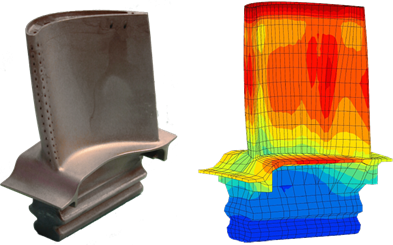
\includegraphics[width=.8\textwidth]{images/rdm}
}%figues de la page de garde

\def\xxpied{%
Cycle 2 -- Modélisation des sollicitations \\
%Ch. 2 : Modélisation des Systèmes Linéaires Continus Invariants -- Transformée de Laplace -- 
\xxactivite%
}


\setcounter{secnumdepth}{5}
%---------------------------------------------------------------------------


\begin{document}
%\chapterimage{png/Fond_Cin}
\pagestyle{empty}


%%%%%%%% PAGE DE GARDE COURS
\ifcours
\begin{tikzpicture}[remember picture,overlay]
\node at (current page.north west)
{\begin{tikzpicture}[remember picture,overlay]
\node[anchor=north west,inner sep=0pt] at (0,0) {\includegraphics[width=\paperwidth]{\thechapterimage}};
\draw[anchor=west] (-2cm,-8cm) node [line width=2pt,rounded corners=15pt,draw=ocre,fill=white,fill opacity=0.6,inner sep=40pt]{\strut\makebox[22cm]{}};
\draw[anchor=west] (1cm,-8cm) node {\huge\sffamily\bfseries\color{black} %
\begin{minipage}{1cm}
\rotatebox{90}{\LARGE\sffamily\textsc{\color{ocre}\textbf{\xxnumpartie}}}
\end{minipage} \hfill
\begin{minipage}[c]{14cm}
\begin{titrepartie}
\begin{flushright}
\renewcommand{\baselinestretch}{1.1} 
\Large\sffamily\textsc{\textbf{\xxpartie}}
\renewcommand{\baselinestretch}{1} 
\end{flushright}
\end{titrepartie}
\end{minipage} \hfill
\begin{minipage}[c]{3.5cm}
{\large\sffamily\textsc{\textbf{\color{ocre} \discipline}}}
\end{minipage} 
 };
\end{tikzpicture}};
\end{tikzpicture}


\begin{tikzpicture}[overlay]
\node[shape=rectangle, 
      rounded corners = .25 cm,
	  draw= ocre,
	  line width=2pt, 
	  fill = ocre!10,
	  minimum width  = 2.5cm,
	  minimum height = 3cm,] at (18cm,0) {};
\node at (17.7cm,0) {\rotatebox{90}{\textbf{\Large\color{ocre}{\classe}}}};
%{};
\end{tikzpicture}

\vspace{3.5cm}

\begin{tikzpicture}[remember picture,overlay]
\draw[anchor=west] (-2cm,-6cm) node {\huge\sffamily\bfseries\color{black} %
\begin{minipage}{2cm}
\begin{center}
\LARGE\sffamily\textsc{\color{ocre}\textbf{\xxactivite}}
\end{center}
\end{minipage} \hfill
\begin{minipage}[c]{15cm}
\begin{titrechapitre}
\renewcommand{\baselinestretch}{1.1} 
\Large\sffamily\textsc{\textbf{\xxnumchapitre}}

\Large\sffamily\textsc{\textbf{\xxchapitre}}
\vspace{.5cm}

\renewcommand{\baselinestretch}{1} 
\normalsize\normalfont
\xxcompetences
\end{titrechapitre}
\end{minipage}  };
\end{tikzpicture}
\vfill

\begin{flushright}
\begin{minipage}[c]{.3\linewidth}
\begin{center}
\xxfigures
\end{center}
\end{minipage}\hfill
\begin{minipage}[c]{.6\linewidth}
\startcontents
\printcontents{}{1}{}
\end{minipage}
\end{flushright}

\begin{tikzpicture}[remember picture,overlay]
\draw[anchor=west] (4.5cm,-.7cm) node {
\begin{minipage}[c]{.2\linewidth}
\begin{flushright}

\includegraphics[width=2cm]{png/logoCC}
\end{flushright}
\end{minipage}
\begin{minipage}[c]{.2\linewidth}
\textsl{\xxauteur} \\
\textsl{\classe}
\end{minipage}
 };
\end{tikzpicture}
\newpage
\pagestyle{fancy}

\newpage
\pagestyle{fancy}

\else
\fi


%%%%%%%% PAGE DE GARDE TD
\iftd
%\begin{tikzpicture}[remember picture,overlay]
%\node at (current page.north west)
%{\begin{tikzpicture}[remember picture,overlay]
%\draw[anchor=west] (-2cm,-3.25cm) node [line width=2pt,rounded corners=15pt,draw=ocre,fill=white,fill opacity=0.6,inner sep=40pt]{\strut\makebox[22cm]{}};
%\draw[anchor=west] (1cm,-3.25cm) node {\huge\sffamily\bfseries\color{black} %
%\begin{minipage}{1cm}
%\rotatebox{90}{\LARGE\sffamily\textsc{\color{ocre}\textbf{\xxnumpartie}}}
%\end{minipage} \hfill
%\begin{minipage}[c]{13.5cm}
%\begin{titrepartie}
%\begin{flushright}
%\renewcommand{\baselinestretch}{1.1} 
%\Large\sffamily\textsc{\textbf{\xxpartie}}
%\renewcommand{\baselinestretch}{1} 
%\end{flushright}
%\end{titrepartie}
%\end{minipage} \hfill
%\begin{minipage}[c]{3.5cm}
%{\large\sffamily\textsc{\textbf{\color{ocre} \discipline}}}
%\end{minipage} 
% };
%\end{tikzpicture}};
%\end{tikzpicture}

%%%%%%%%%% PAGE DE GARDE TD %%%%%%%%%%%%%%%
%\begin{tikzpicture}[overlay]
%\node[shape=rectangle, 
%      rounded corners = .25 cm,
%	  draw= ocre,
%	  line width=2pt, 
%	  fill = ocre!10,
%	  minimum width  = 2.5cm,
%	  minimum height = 2.5cm,] at (18.5cm,0) {};
%\node at (17.7cm,0) {\rotatebox{90}{\textbf{\Large\color{ocre}{\classe}}}};
%%{};
%\end{tikzpicture}

% PARTIE ET CHAPITRE
%\begin{tikzpicture}[remember picture,overlay]
%\draw[anchor=west] (-1cm,-2.1cm) node {\large\sffamily\bfseries\color{black} %
%\begin{minipage}[c]{15cm}
%\begin{flushleft}
%\xxnumchapitre \\
%\xxchapitre
%\end{flushleft}
%\end{minipage}  };
%\end{tikzpicture}

% Bandeau titre exo
\begin{tikzpicture}[remember picture,overlay]
\draw[anchor=west] (-2cm,-6cm) node {\huge\sffamily\bfseries\color{black} %
\begin{minipage}{5cm}
\begin{center}
\LARGE\sffamily\color{ocre}\textbf{\textsc{\xxactivite}}

\begin{center}
\xxfigures
\end{center}

\end{center}
\end{minipage} \hfill
\begin{minipage}[c]{12cm}
\begin{titrechapitre}
\renewcommand{\baselinestretch}{1.1} 
\large\sffamily\textbf{\textsc{\xxtitreexo}}

\small\sffamily{\textbf{\textit{\color{black!70}\xxsourceexo}}}
\vspace{.5cm}

\renewcommand{\baselinestretch}{1} 
\normalsize\normalfont
\xxcompetences
\end{titrechapitre}
\end{minipage}  };
\end{tikzpicture}

\else
\fi


%%%%%%%% PAGE DE GARDE FICHE
\iffiche
\begin{tikzpicture}[remember picture,overlay]
\node at (current page.north west)
{\begin{tikzpicture}[remember picture,overlay]
\draw[anchor=west] (-2cm,-3.25cm) node [line width=2pt,rounded corners=15pt,draw=ocre,fill=white,fill opacity=0.6,inner sep=40pt]{\strut\makebox[22cm]{}};
\draw[anchor=west] (1cm,-3.25cm) node {\huge\sffamily\bfseries\color{black} %
\begin{minipage}{1cm}
\rotatebox{90}{\LARGE\sffamily\textsc{\color{ocre}\textbf{\xxnumpartie}}}
\end{minipage} \hfill
\begin{minipage}[c]{14cm}
\begin{titrepartie}
\begin{flushright}
\renewcommand{\baselinestretch}{1.1} 
\large\sffamily\textsc{\textbf{\xxpartie} \\} 

\vspace{.2cm}

\normalsize\sffamily\textsc{\textbf{\xxnumchapitre -- \xxchapitre}}
\renewcommand{\baselinestretch}{1} 
\end{flushright}
\end{titrepartie}
\end{minipage} \hfill
\begin{minipage}[c]{3.5cm}
{\large\sffamily\textsc{\textbf{\color{ocre} \discipline}}}
\end{minipage} 
 };
\end{tikzpicture}};
\end{tikzpicture}


\begin{tikzpicture}[overlay]
\node[shape=rectangle, 
      rounded corners = .25 cm,
	  draw= ocre,
	  line width=2pt, 
	  fill = ocre!10,
	  minimum width  = 2.5cm,
%	  minimum height = 2.5cm,] at (18.5cm,0.5cm) {};
	  minimum height = 2.5cm,] at (18.5cm,0cm) {};
\node at (17.7cm,0) {\rotatebox{90}{\textsf{\textbf{\large\color{ocre}{\classe}}}}};
%{};
\end{tikzpicture}



\else
\fi



\vspace{7cm}
\pagestyle{fancy}
\thispagestyle{plain}


\def\columnseprulecolor{\color{ocre}}
\setlength{\columnseprule}{0.4pt} 
\ifprof
\else
\begin{multicols}{2}
\fi

\section*{Exercice 1}
\setcounter{subparagraph}{0}
On donne sur le schéma ci-dessous la modélisation d'une poutre et des efforts qui lui sont appliqués.
\begin{center}
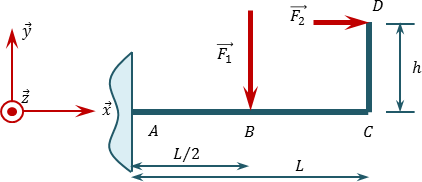
\includegraphics[width=.45\textwidth]{images/exo_08}
\end{center}

\subparagraph{}
\textit{Proposer une méthode permettant de déterminer le torseur de cohésion dans chacun des tronçons. Est-il nécessaire de déterminer les actions mécaniques en $A$ ?}

\subparagraph{}
\textit{Déterminer le torseur de cohésion dans chacun des tronçons.}


\ifprof
\begin{corrige}
\subsubsection*{On considère le tronçon AB}
On considère donc $\vect{AG} = \lambda \vect{x}$ avec $\lambda\in \left[0,\dfrac{L}{2}\right]$.
\begin{center}
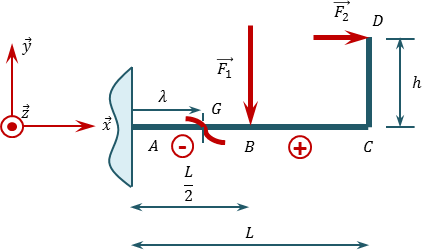
\includegraphics[width=.45\textwidth]{images/exo_08_corr_01}
\end{center}


On isole la partie de droite, notée $+$ soumise aux actions de :
\begin{itemize}[label=\ding{112},font=\color{ocre}] 
\item torseur de cohésion : $\torseurscoh_{S-\rightarrow S+}$ en $G$;
\item action mécanique en $B$ : $\torseurcol{0}{-F_1}{0}{0}{0}{0}{B,\left( \vect{x},\vect{y},\vect{z} \right)}  =\torseurcol{0}{-F_1}{0}{0}{0}{-\left(\dfrac{L}{2}-\lambda \right)F_1}{G,\left( \vect{x},\vect{y},\vect{z} \right)} $;
\item action mécanique en $D$ : $\torseurcol{F_2}{0}{0}{0}{0}{0}{D,\left( \vect{x},\vect{y},\vect{z} \right)}  =\torseurcol{F_2}{0}{0}{0}{0}{-F_2h}{G,\left( \vect{x},\vect{y},\vect{z} \right)} $.
\end{itemize}


Par application du PFS on a : 
$$ \torseurscoh_{S-\rightarrow S+} +\torseurstat{T}{F_1}{S+} +\torseurstat{T}{F_2}{S+} = \{0\} \Leftrightarrow \torseurscoh_{S+\rightarrow S-} =\torseurstat{T}{F_1}{S+} +\torseurstat{T}{F_2}{S+}  $$
On a donc  :
$$
\torseurcol{N}{T_y}{T_z}{M_t}{Mf_y}{Mf_z}{G} = 
\torseurcol{F_2}{-F_1}{0}{0}{0}{-\left(\dfrac{L}{2}-\lambda \right)F_1-F_2h}{G,\left( \vect{x},\vect{y},\vect{z} \right)}
$$

\subsubsection*{On considère le tronçon BC}
On considère donc $\vect{AG} = \lambda \vect{x}$ avec $\lambda\in \left[\dfrac{L}{2},L\right]$.
\begin{center}
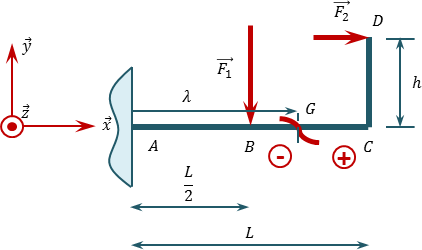
\includegraphics[width=.45\textwidth]{images/exo_08_corr_02}
\end{center}


On isole la partie de droite, notée $+$ soumise aux actions de :
\begin{itemize}[label=\ding{112},font=\color{ocre}] 
\item torseur de cohésion : $\torseurscoh_{S-\rightarrow S+}$ en $G$;
\item action mécanique en $D$ : $\torseurcol{F_2}{0}{0}{0}{0}{0}{D,\left( \vect{x},\vect{y},\vect{z} \right)}  =\torseurcol{F_2}{0}{0}{0}{0}{-F_2h}{G,\left( \vect{x},\vect{y},\vect{z} \right)} $.
\end{itemize}


Par application du PFS on a : 
$$ \torseurscoh_{S-\rightarrow S+} +\torseurstat{T}{F_2}{S+} = \{0\} \Leftrightarrow \torseurscoh_{S+\rightarrow S-} =\torseurstat{T}{F_2}{S+}  $$
On a donc  :
$$
\torseurcol{N}{T_y}{T_z}{M_t}{Mf_y}{Mf_z}{G} = 
\torseurcol{F_2}{0}{0}{0}{0}{-F_2h}{G,\left( \vect{x},\vect{y},\vect{z} \right)}
$$
\subsubsection*{On considère le tronçon CD}
On considère donc $\vect{AG} = \lambda \vect{x}_1-L \vect{y}_1$  avec $\lambda\in \left[0,h\right]$.
\begin{center}
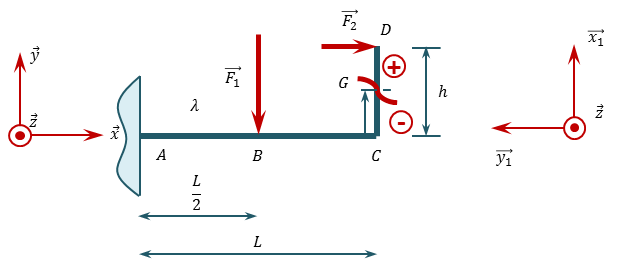
\includegraphics[width=.45\textwidth]{images/exo_08_corr_03}
\end{center}


On isole la partie de droite, notée $+$ soumise aux actions de :
\begin{itemize}[label=\ding{112},font=\color{ocre}] 
\item torseur de cohésion : $\torseurscoh_{S-\rightarrow S+}$ en $G$;
\item action mécanique en $D$ : $\torseurcol{0}{-F_2}{0}{0}{0}{0}{D,\left( \vect{x_1},\vect{y_1},\vect{z} \right)}  =\torseurcol{0}{-F_2}{0}{0}{0}{-F_2\left(h-\lambda\right)}{G,\left( \vect{x_1},\vect{y_1},\vect{z} \right)} $.
\end{itemize}


Par application du PFS on a : 
$$ \torseurscoh_{S-\rightarrow S+} +\torseurstat{T}{F_2}{S+} = \{0\} \Leftrightarrow \torseurscoh_{S+\rightarrow S-} =+\torseurstat{T}{F_2}{S+}  $$
On a donc  :
$$
\torseurcol{N}{T_y}{T_z}{M_t}{Mf_y}{Mf_z}{G,\left( \vect{x_1},\vect{y_1},\vect{z} \right)} = 
\torseurcol{0}{-F_2}{0}{0}{0}{-F_2\left(h-\lambda\right)}{G,\left( \vect{x_1},\vect{y_1},\vect{z} \right)}
$$



\end{corrige}
\else 
\fi


\subparagraph{}
\textit{Tracer le diagramme des sollicitations.}



\section*{Exercice 2}
\setcounter{subparagraph}{0}
On donne sur le schéma ci-dessous la modélisation d'une poutre et des efforts qui lui sont appliqués.
\subparagraph{}
\textit{Est-il nécessaire de déterminer les actions mécaniques en $A$ et en $B$.}
\ifprof
\begin{corrige}
Si on isole la partie <<II>>, elle est soumise à l'effort $\vect{F}$ et à l'action du torseur de cohésion. On n'aura donc pas besoin de l'action dans la liaison encastrement pour pouvoir déterminer le torseur de cohésion. 
\end{corrige}
\else 
\fi


On cherche à déterminer le diagramme des sollicitations dans chacun des tronçons.

\subparagraph{}
\textit{Exprimer le torseur de cohésion dans chacun des tronçons.}
\ifprof
\begin{corrige}
 ~\\
\begin{itemize}[label=\ding{112},font=\color{ocre}] 
\item On isole la portion $[MB]$ (+).
\item La portion est soumise d'une part à l'action mécanique en $B$ et d'autre part à l'action mécanique du torseur de cohésion.
\item On a donc : 
\end{itemize}
$$
\torseurscoh_{S-\rightarrow S+} +
 \torseurcol{-F}{0}{0}{0}{0}{0}{B,\left( \vect{x},\vect{y},\vect{z} \right)} 
 = \{0\}
$$
%
%$$
%\torseurscoh_{S+\rightarrow S-}
%=-\torseurcol{F}{0}{0}{0}{0}{0}{G}
%-\torseurcol{0}{-px}{0}{0}{0}{ \dfrac{px^2}{2}}{G}
%=\torseurcol{-F}{px}{0}{0}{0}{-\dfrac{px^2}{2}}{G}
%$$
%car 
$\vectm{M}{\text{Ext}}{\text{Poutre}}
=\vectm{B}{\text{Ext}}{\text{Poutre}} + \vect{MB}  \wedge -F \vect{x} 
=\left( -R\vect{u} + R\vect{x}\right) \wedge -F \vect{x} 
=  - RF \sin \theta \vect{z}
$  et $-F \vect{x}  = -F \left( \cos \theta \vect{u}-\sin \theta \vect{v} \right) $.

On a donc :
$$
\torseurscoh_{S+\rightarrow S-} 
= 
 \torseurcol{-F\cos \theta }{F\sin \theta }{0}{0}{0}{ - RF \sin \theta}{M,\left( \vect{u},\vect{v},\vect{z} \right)} 
$$

\textbf{TODO : diagrammes}
\end{corrige}
\else 
\fi


%\subparagraph{}
%\textit{Tracer les diagrammes des sollicitations.}
%\ifprof
%\begin{corrige}
%\end{corrige}
%\else 
%\fi
\ifprof
\else
\begin{center}
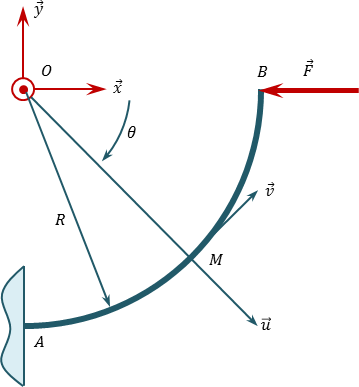
\includegraphics[width=.4\textwidth]{images/exo_04}
\end{center}
\fi


\section*{Exercice 3}
\setcounter{subparagraph}{0}
On donne sur le schéma ci-dessous la modélisation d'une poutre et des efforts qui lui sont appliqués. On note $p$ la densité d'effort linéique.
\begin{center}
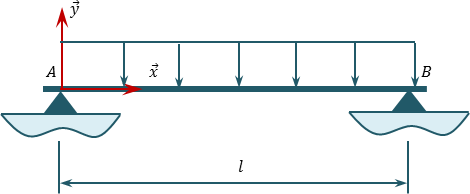
\includegraphics[width=.45\textwidth]{images/exo_05}
\end{center}

\subparagraph{}
\textit{Déterminer les actions mécaniques en $A$ et en $B$.}
\ifprof
\begin{corrige}
On a $Y_A = Y_B = \dfrac{pl}{2}$.
\end{corrige}
\else 
\fi


%On cherche à déterminer le diagramme des sollicitations dans chacun des tronçons.

\subparagraph{}
\textit{Exprimer le torseur de cohésion dans chacun des tronçons.}
\ifprof
\begin{corrige}
\begin{itemize}
\item On isole la portion $[GB]$.
\item La portion est soumise à l'action mécanique en $B$, à l'action uniformément répartie (exprimée en $M$, milieu de $[GB]$) et à l'action mécanique du torseur de cohésion en $G$.
\item On a donc : 
\end{itemize}
$$
\torseurscoh_{S-\rightarrow S+} +
 \torseurcol{0}{\dfrac{pl}{2}}{0}{0}{0}{0}{B,\left( \vect{x},\vect{y},\vect{z} \right)} 
 +\torseurcol{0}{-p(l-x)}{0}{0}{0}{0}{M,\left( \vect{x},\vect{y},\vect{z} \right)} 
 = \{0\}
$$
On a donc, $\forall x \in \left[0,l\right]$, 
$$
\torseurscoh_{S+\rightarrow S-}
= \torseurcol{0}{\dfrac{pl}{2}}{0}{0}{0}{(l-x)\dfrac{pl}{2}}{G} 
 +\torseurcol{0}{-p(l-x)}{0}{0}{0}{-p\dfrac{\left(l-x\right)^2}{2}}{G} 
 = \torseurcol{0}{\dfrac{pl}{2}-p(l-x)}{0}{0}{0}{(l-x)\dfrac{pl}{2}-p\dfrac{\left(l-x\right)^2}{2}}{G} 
$$
car 
$\vectm{G}{\text{Ext}}{\text{Poutre}}
=\vectm{B}{\text{Ext}}{\text{Poutre}} + \vect{GB}\wedge \dfrac{pl}{2} \vect{y}  
=  (l-x)\vect{x}  \wedge \dfrac{pl}{2} \vect{y}
=  \dfrac{pl(l-x)}{2} \vect{z}
$ 

et 
$\vectm{G}{\text{Ext}}{\text{Poutre}}
=  \vectm{M}{\text{Ext}}{\text{Poutre}} + \vect{GM}\wedge \left( -p(l-x) \right) \vect{y}  
= \left(\dfrac{l-x}{2}\right)\vect{x}\wedge \left(-p(l-x)\right) \vect{y}  
=  -p\dfrac{\left(l-x\right)^2}{2}\vect{z}  
$.
\end{corrige}
\else 
\fi

\subparagraph{}
\textit{Tracer les diagrammes des sollicitations.}
\ifprof
\begin{corrige}
\end{corrige}
\else 
\fi

%\newpage

\section*{Exercice 5}
\setcounter{subparagraph}{0}
On donne sur le schéma ci-dessous la modélisation d'une poutre. On y exerce une charge répartie de pression $p$ (en $\text{N}\text{m}^{-1}$).
\begin{center}
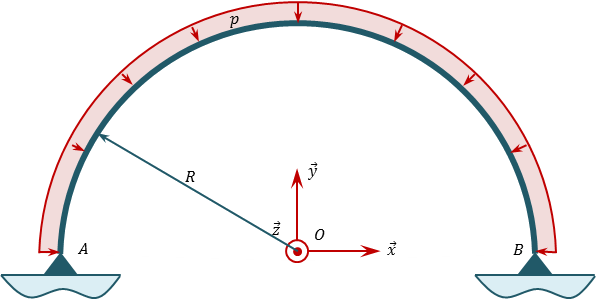
\includegraphics[width=.45\textwidth]{images/exo_06}
\end{center}

\subparagraph{}
\textit{Déterminer les actions mécaniques en $A$ et en $B$.}
\ifprof
\begin{corrige}
L'action de pression est modélisable par le glisseur suivant : 
$$\mathcal{T}_{\text{Pression}\rightarrow \text{Poutre}} =\torseurl{\vectf{\text{Pr}}{\text{Po}}=- 2 p R \vect{y}=-F\vect{y}}{\vectm{O}{\text{Pr}}{\text{Po}}=\vect{0}}{O}$$

On a donc :
$$\mathcal{T}_{\text{Ext}\rightarrow \text{Poutre A}} =\torseurl{\vectf{\text{Ext}}{\text{Po A}}=\dfrac{1}{2}F\vect{y}}{\vectm{O}{\text{Pr}}{\text{Po A}}=\vect{0}}{O}$$

$$\mathcal{T}_{\text{Ext}\rightarrow \text{Poutre B}} =\torseurl{\vectf{\text{Ext}}{\text{Po B}}=\dfrac{1}{2}F\vect{y}}{\vectm{O}{\text{Pr}}{\text{Po B}}=\vect{0}}{O}$$



\end{corrige}
\else 
\fi


On cherche à déterminer le diagramme des sollicitations dans chacun des tronçons.

\subparagraph{}
\textit{Quels tronçons peut-on considérer ?}
\ifprof
\begin{corrige}
On ne considèrera qu'une seule partie, dans laquelle on aura deux tronçons.

\begin{center}
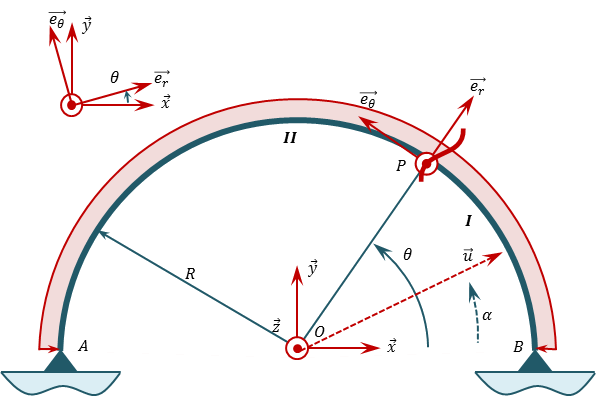
\includegraphics[width=.9\textwidth]{images/exo_06_param}
\end{center}

\end{corrige}
\else 
\fi

\subparagraph{}
\textit{Exprimer le torseur de cohésion dans chacun des tronçons, de préférence dans une base locale.}

\ifprof
\begin{corrige}
Pour $\theta \in \left[0 ;  \pi \right]$, en appliquant le théorème de la résultante statique sur le tronçon $I$ on a : 
%$$
%\torseurscoh_{II \rightarrow I} 
%+\left\{\mathcal{T}_{\text{Ext}\rightarrow \text{Poutre B}}\right\} 
%+\left\{\mathcal{T}_{\text{Pression}\rightarrow \text{Poutre}} \right\}  = \{0\}
%$$

$$
\torseurscoh_{II \rightarrow I} 
+\left\{\mathcal{T}_{\text{Ext}\rightarrow I}\right\} 
+\left\{\mathcal{T}_{\text{Pression}\rightarrow I} \right\}  = \{0\}
$$
\end{corrige}

\begin{corrige}
Exprimons $\left\{\mathcal{T}_{\text{Ext}\rightarrow \text{I}}\right\} $ au point $P$ : 

$$\left\{\mathcal{T}_{\text{Ext}\rightarrow \text{I}}\right\} 
=\torseurl{\vectf{\text{Ext}}{\text{I}} }{\vectm{P}{\text{Ext}}{\text{I}} }{P}
$$

\begin{itemize}
\item $\vectf{\text{Ext}}{\text{I}} =\dfrac{1}{2}F\vect{y} = \dfrac{1}{2}F\left( \sin\theta \vect{e_r} + \cos\theta \vect{e_\theta} \right) $ 

$\vectf{\text{Ext}}{\text{I}} = pR\left( \sin\theta \vect{e_r} + \cos\theta \vect{e_\theta} \right) $ 

\item $\vectm{P}{\text{Ext}}{\text{I}} $


$= \vectm{B}{\text{Ext}}{\text{I}} + \vect{PB} \wedge \vectf{\text{Ext}}{\text{I}}$

$= \left( -R \vect{e_r} +R \vect{x} \right) \wedge\dfrac{1}{2}F\vect{y}$

$= \left( -R \cos \theta \vect{x} -R \sin \theta \vect{y} +R \vect{x} \right) \wedge\dfrac{1}{2}F\vect{y}$

$= \dfrac{1}{2}F \left( -R \cos \theta  +R \right)\vect{z}$

$= \dfrac{RF}{2} \left( 1- \cos \theta \right)\vect{z}$

$= pR^2 \left( 1- \cos \theta \right)\vect{z}$.


$$\left\{\mathcal{T}_{\text{Ext}\rightarrow \text{I}}\right\} 
=\torseurl{ 
 pR\left( \sin\theta \vect{e_r} + \cos\theta \vect{e_\theta} \right)}{
pR^2 \left( 1- \cos \theta \right)\vect{z}} {P}
$$

%\item $\vectm{O}{\text{Ext}}{\text{I}} $
%
%
%$= \vectm{B}{\text{Ext}}{\text{I}} + \vect{OB} \wedge \vectf{\text{Ext}}{\text{I}}$
%
%$=  R \vect{x}  \wedge\dfrac{1}{2}F\vect{y}=\dfrac{RF}{2}\vect{z}$.
\end{itemize}

\end{corrige}

\begin{corrige}
Exprimons $\left\{\mathcal{T}_{\text{Pression}\rightarrow \text{I}}\right\} $ au point $O$.

$$\left\{\mathcal{T}_{\text{Pr}\rightarrow \text{I}}\right\} 
=\torseurl{\vectf{\text{Pr}}{\text{I}} }{\vectm{O}{\text{Pr}}{\text{I}} = \vect{0} }{O} 
$$

\begin{itemize}
\item $\vectf{\text{Pr}}{\text{I}} = \int_0^{\theta} pR (-\vect{e_r})\text{d}\alpha $

$= -pR \left( \left[ \sin \alpha \right]_0^\theta \vect{x} - \left[ \cos\alpha  \right]_0^\theta \vect{y}\right)$

$= -pR \left( \sin \theta \vect{x} - \left( \cos\theta -1  \right) \vect{y}\right)$

$= -pR \left( \sin \theta \left( \cos\theta\vect{e_r} - \sin\theta \vect{e_\theta} \right) \right. $

$\left.- \left( \cos\theta -1  \right) \left(  \cos\theta\vect{e_\theta} + \sin\theta \vect{e_r} \right)\right)$

$= -pR \left( \sin \theta\cos\theta\vect{e_r} - \sin^2\theta \vect{e_\theta}  +    \cos\theta\vect{e_\theta} \right.$

$\left. + \sin\theta \vect{e_r} - \cos^2\theta\vect{e_\theta} - \cos\theta\sin\theta \vect{e_r} \right)$

$= -pR \left(   \sin\theta \vect{e_r}  +\left( \cos\theta -1 \right) \vect{e_\theta}  \right)$



$$\left\{\mathcal{T}_{\text{Pr}\rightarrow \text{I}}\right\} 
=\torseurl{-pR \left(   \sin\theta \vect{e_r}  +\left( \cos\theta -1 \right) \vect{e_\theta}  \right) }{\vect{0} }{O} 
$$

%$= pR \left( - \sin ^2\theta \vect{e_r}  -\cos^2 \theta\vect{e_\theta}  + \cos\theta \vect{e_\theta} + \sin\theta \vect{e_r} \right)$


%
%$- pR\theta \cos\dfrac{\theta}{2} \vect{x}- pR\theta \sin\dfrac{\theta}{2} \vect{y}$
%
%$=- pR\theta \cos\dfrac{\theta}{2} \left(\cos \theta  \vect{e_r} - \sin \theta  \vect{e_\theta}   \right) $
%
%$- pR\theta \sin\dfrac{\theta}{2}  \left( \cos \theta  \vect{e_\theta} +\sin \theta  \vect{e_r}   \right) $
%
%$ = - pR\theta \cos\dfrac{\theta}{2} \cos \theta  \vect{e_r} + pR\theta \cos\dfrac{\theta}{2} \sin \theta  \vect{e_\theta}   $
%
%$
%- pR\theta \sin\dfrac{\theta}{2} \cos \theta  \vect{e_\theta} 
%- pR\theta \sin\dfrac{\theta}{2} \sin \theta  \vect{e_r}  
%$
%
%$
%= - pR\theta\left(\cos\dfrac{\theta}{2} \cos \theta   + \sin\dfrac{\theta}{2} \sin \theta \right) \vect{e_r}
%$
%
%$
%+pR\theta  \left( \cos\dfrac{\theta}{2} \sin \theta  
%- \sin\dfrac{\theta}{2} \cos \theta    \right)\vect{e_\theta}
%$
%
%$
%= - pR\theta\left(\cos\dfrac{\theta}{2} \right) \vect{e_r}
%+pR\theta  \left( \sin\dfrac{\theta}{2}  \right)\vect{e_\theta}
%$

\end{itemize}
\end{corrige}

\begin{corrige}
Exprimons $\left\{\mathcal{T}_{\text{Pression}\rightarrow \text{I}}\right\} $ au point $P$.

$$\left\{\mathcal{T}_{\text{Pr}\rightarrow \text{I}}\right\} 
=\torseurl{\vectf{\text{Pr}}{\text{I}} }{\vectm{P}{\text{Pr}}{\text{I}} }{P} 
$$


$\vectm{P}{\text{Pr}}{\text{I}} = \vectm{O}{\text{Pr}}{I} + \vect{PO} \wedge\vectf{\text{Pr}}{\text{I}} $

$ = -R\vect{e_r}\wedge \left(  -pR \left(   \sin\theta \vect{e_r}  +\left( \cos\theta -1 \right) \vect{e_\theta}  \right)\right)$

$ = pR^2 \left( \cos\theta -1 \right) \vect{z}$




$$\left\{\mathcal{T}_{\text{Pr}\rightarrow \text{I}}\right\} 
=\torseurl{-pR \left(   \sin\theta \vect{e_r}  +\left( \cos\theta -1 \right) \vect{e_\theta}  \right) }{pR^2 \left( \cos\theta -1 \right) \vect{z} }{P} 
$$

\end{corrige}





\begin{corrige}

En conclusion, 
$$
\torseurscoh_{II \rightarrow I} 
+\left\{\mathcal{T}_{\text{Ext}\rightarrow I}\right\} 
+\left\{\mathcal{T}_{\text{Pression}\rightarrow I} \right\}  = \{0\}
$$

$$
\torseurscoh_{II \rightarrow I}
= 
-\left\{\mathcal{T}_{\text{Ext}\rightarrow I}\right\} 
-\left\{\mathcal{T}_{\text{Pression}\rightarrow I} \right\}  
$$

$$
\torseurscoh_{II \rightarrow I}
= 
-\torseurl{ 
 pR\left( \sin\theta \vect{e_r} + \cos\theta \vect{e_\theta} \right)}{
pR^2 \left( 1- \cos \theta \right)\vect{z}} {P}
-\torseurl{-pR \left(   \sin\theta \vect{e_r}  +\left( \cos\theta -1 \right) \vect{e_\theta}  \right) }{pR^2 \left( \cos\theta -1 \right) \vect{z} }{P} 
$$



$$
\torseurscoh_{II \rightarrow I}
= 
\torseurl{ 
 -pR\left( \sin\theta \vect{e_r} + \cos\theta \vect{e_\theta} \right) +pR \left(   \sin\theta \vect{e_r}  +\left( \cos\theta -1 \right) \vect{e_\theta}  \right) }{
-pR^2 \left( 1- \cos \theta \right)\vect{z} - pR^2 \left( \cos\theta -1 \right) } {P}
$$


$$
\torseurscoh_{II \rightarrow I}
= 
\torseurl{ 
-pR  \vect{e_\theta}  }{
\vect{0} } {P}
$$

\end{corrige}
\else
\fi





\newpage



\section*{Exercice 1}
\setcounter{subparagraph}{0}
On donne sur le schéma ci-dessous la modélisation d'une poutre et des efforts qui lui sont appliqués.
\begin{center}
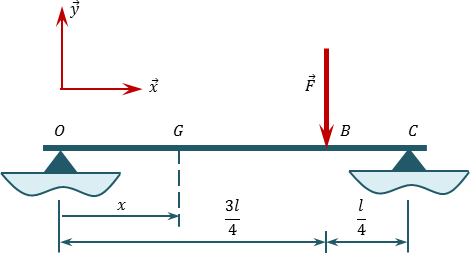
\includegraphics[width=.45\textwidth]{images/exo_01}
\end{center}

\subparagraph{}
\textit{Déterminer les actions mécaniques en $A$ et en $B$.}
\ifprof
\begin{corrige}~\\

\begin{itemize}[label=\ding{112},font=\color{ocre}] 
\item On isole la poutre.
\item On réalise le bilan des actions mécaniques :
\begin{itemize}[label=\ding{110},font=\color{ocre} \footnotesize] 
\item liaison sphère-plan en $O$. Sans frottement, cette action est de direction $\vect{y}$;
\item liaison sphère-plan en $C$. Sans frottement, cette action est de direction $\vect{y}$;
\item action mécanique en $B$.
\end{itemize}
\item On réalise un théorème de la résultante statique en $C$ en projection sur $\vect{y}$ et un théorème du moment statique appliqué au point $O$ en projection suivant $\vect{z}$ :
$$
\left\{
\begin{array}{l}
Y_O + Y_C -F = 0 \\
-\dfrac{3l}{4}F + l Y_C = 0 \\
\end{array}
\right.
\Leftrightarrow
\left\{
\begin{array}{l}
Y_O = F -  \dfrac{3}{4}F  = \dfrac{F}{4} \\
Y_C = \dfrac{3}{4}F \\
\end{array}
\right.
$$
\end{itemize}

\end{corrige}
\else 
\fi
On cherche à déterminer le diagramme des sollicitations dans chacun des tronçons.

\subparagraph{}
\textit{Quels tronçons peut-on considérer ?}
\ifprof
\begin{corrige}
Dans le cadre de cette étude on considèrera les tronçons suivants : $x\in\left[0,\dfrac{3l}{4}\right]$ et $x\in\left[\dfrac{3l}{4},l\right]$.

\end{corrige}
\else 
\fi

\subparagraph{}
\textit{Exprimer le torseur de cohésion dans chacun des tronçons.}
\ifprof
\begin{corrige}~\\
\begin{itemize}[label=\ding{112},font=\color{ocre}] 
\item On isole le premier tronçon.
\item Le tronçon est soumis d'une part à l'action mécanique en $O$ et d'autre part à l'action mécanique du torseur de cohésion.
\item On a donc :
\end{itemize}
$$
\torseurscoh_{S+\rightarrow S-} + \torseurcol{0}{Y_O}{0}{0}{0}{0}{A,\left( \vect{x},\vect{y},\vect{z} \right)} = \{0\}
$$
On a donc :
$$\torseurscoh_{S+\rightarrow S-}
=-\torseurcol{0}{Y_O}{0}{0}{0}{0}{A}
=\torseurcol{0}{-\dfrac{F}{4}}{0}{0}{0}{ \dfrac{F}{4}x}{G}
$$
car $\vectm{G}{\text{Ext}}{\text{Poutre}}=\vectm{O}{\text{Ext}}{\text{Poutre}} + \vect{GO}\wedge Y_O \vect{y}  = -x\vect{x} \wedge Y_O \vect{y} = -x Y_O \vect{z}= -x \dfrac{F}{4} \vect{z}$.
%\end{corrige}

%\begin{corrige}
\begin{itemize}[label=\ding{112},font=\color{ocre}] 
\item On isole le second tronçon.
\item Le tronçon est soumis d'une part à l'action mécanique en $C$ et d'autre part à l'action mécanique du torseur de cohésion.
\item On a donc :
\end{itemize}
$$
\torseurscoh_{S-\rightarrow S+} + \torseurcol{0}{Y_C}{0}{0}{0}{0}{A,\left( \vect{x},\vect{y},\vect{z} \right)} = \{0\}
$$
On a donc, $\forall x \in\left[\dfrac{3l}{4},l\right]$ :
$$
\torseurscoh_{S-\rightarrow S+}
=-\torseurcol{0}{Y_C}{0}{0}{0}{0}{A}
=-\torseurcol{0}{\dfrac{3F}{4}}{0}{0}{0}{ (l-x) \dfrac{3F}{4}}{G}
$$
car $\vectm{G}{\text{Ext}}{\text{Poutre}}=\vectm{C}{\text{Ext}}{\text{Poutre}} + \vect{GC}\wedge Y_C \vect{y}  = (l-x)\vect{x} \wedge Y_C \vect{y} = (l-x) Y_C \vect{z}= (l-x) \dfrac{3F}{4} \vect{z}$.

Au final,
$$\torseurscoh_{S+\rightarrow S-}
=\torseurcol{0}{\dfrac{3F}{4}}{0}{0}{0}{ (l-x) \dfrac{3F}{4}}{G}
$$
\end{corrige}
\else 
\fi

\subparagraph{}
\textit{Tracer les diagrammes des sollicitations.}
\ifprof
\begin{corrige}~\\

\begin{center}
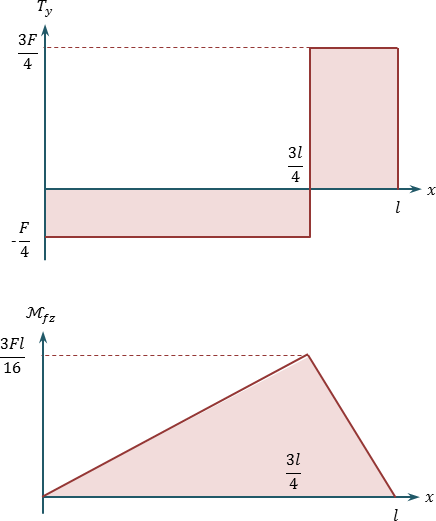
\includegraphics[width=.5\textwidth]{images/exo_01_corr}
\end{center}
\end{corrige}
\else 
\fi



\section*{Exercice 2}
\setcounter{subparagraph}{0}
On donne sur le schéma ci-dessous la modélisation d'une poutre et des efforts qui lui sont appliqués.
\begin{center}
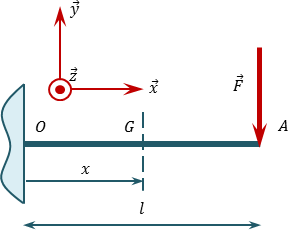
\includegraphics[width=.45\textwidth]{images/exo_01_01}
\end{center}

\subparagraph{}
\textit{Donner une méthode permettant de déterminer le torseur de cohésion sans calculer les actions mécaniques en $O$.}
\ifprof
\begin{corrige} Si on isole la partie comprise entre $G$ et $A$ et qu'on applique le PFS, cette partie est soumise aux efforts de cohésion et à l'action mécanique en $A$. Il n'est donc pas nécessaire de déterminer les efforts en $O$.
\end{corrige}
\else
\fi

\subparagraph{}
\textit{Exprimer le torseur de cohésion.}
\ifprof
\begin{corrige} ~\\
\begin{minipage}[c]{.48\linewidth}
\begin{itemize}[label=\ding{112},font=\color{ocre}] 
\item On isole la portion comprise entre $G$ et $A$.
\item Cette partie est soumises aux actions mécaniques de l'effort en $A$ et des actions du torseur de cohésion. 
\item On réalise le PFS sur cette partie et on a :
\end{itemize}
\end{minipage} \hfill
\begin{minipage}[c]{.48\linewidth}
\begin{center}
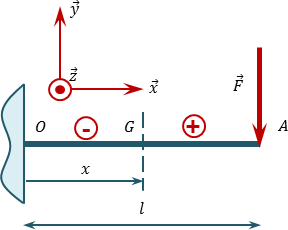
\includegraphics[width=.85\linewidth]{images/exo_01_01_corr_01}
\end{center}
\end{minipage} 

$$
\torseurscoh_{S-\rightarrow S+} + \torseurcol{0}{0}{-F}{0}{0}{0}{A,\left( \vect{x},\vect{y},\vect{z} \right)} = \{0\}
$$
On a donc, $\forall x \in\left[0,l\right]$ :
$$
\torseurscoh_{S+\rightarrow S-}
=\torseurcol{0}{0}{-F}{0}{0}{0}{A,\left( \vect{x},\vect{y},\vect{z} \right)}
=\torseurcol{0}{0}{-F}{0}{0}{(x-l) F}{G,\left( \vect{x},\vect{y},\vect{z} \right)}
=\torseurcol{N}{T_y}{T_z}{\mathcal{M}_t}{\mathcal{M}_{fy}}{\mathcal{M}_{fz}}{G}
$$
car $\vectm{G}{\text{Ext}}{\text{Poutre}}=\vectm{A}{\text{Ext}}{\text{Poutre}} + \vect{GA}\wedge - F \vect{y}  = (l-x)\vect{x} \wedge -F \vect{y} = (x-l) F \vect{z}$.

\end{corrige}
\else
\fi

\subparagraph{}
\textit{Tracer les diagrammes des sollicitations.}
\ifprof
\begin{corrige}~\\

\begin{center}
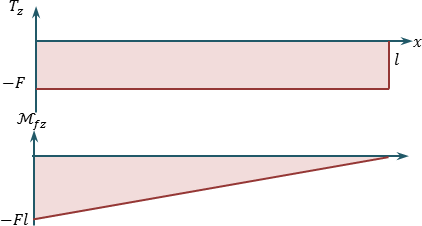
\includegraphics[width=.6\linewidth]{images/exo_01_01_corr_02}
\end{center}
\end{corrige}
\else
\fi

\section*{Exercice 3}
\setcounter{subparagraph}{0}
On donne sur le schéma ci-dessous la modélisation d'une poutre et des efforts qui lui sont appliqués.
\begin{center}
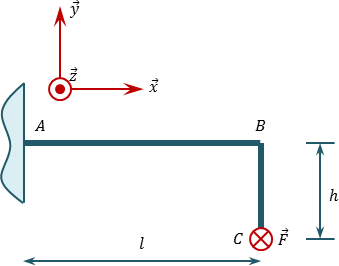
\includegraphics[width=.45\textwidth]{images/exo_02}
\end{center}

\subparagraph{}
\textit{Déterminer les actions mécaniques en $A$ et en $B$... et remarquer que cela peut ne servir à rien pour la suite du problème...}
\ifprof
\begin{corrige}
\textit{Remarque :}
Pour déterminer le torseur de cohésion dans ce cas il n'est pas nécessaire de déterminer les actions mécaniques dans la liaison encastrement.

\begin{itemize}[label=\ding{112},font=\color{ocre}] 
\item On isole la poutre.
\item La poutre est soumise à une liaison encastrement en $A$ et à une action mécanique en $C$.
\item On a donc :
\end{itemize}
$$
\torseurcol{X_A}{Y_A}{Z_A}{L_A}{M_A}{N_A}{A}
+\torseurcol{0}{0}{-F}{0}{0}{0}{C}
=\{ 0\}
$$

$\vectm{A}{\text{Ext}}{\text{Poutre}}
=\vectm{C}{\text{Ext}}{\text{Poutre}} + \vect{AC}\wedge -F \vect{z}  
= \left(l\vect{x} - h\vect{z} \right) \wedge -F \vect{z}  
= Fl\vect{y}$

$$
\torseurcol{X_A}{Y_A}{Z_A}{L_A}{M_A}{N_A}{A}
= \torseurcol{0}{0}{F}{0}{-Fl}{0}{A}
$$

\end{corrige}
\else 
\fi


On cherche à déterminer le diagramme des sollicitations dans chacun des tronçons.

\subparagraph{}
\textit{Quels tronçons peut-on considérer ?}
\ifprof
\begin{corrige}~\\
\begin{minipage}[c]{.45\linewidth}
On peut considérer les deux tronçons suivants :
\begin{itemize}[label=\ding{112},font=\color{ocre}] 
\item le tronçon $AB$ sur lequel $x\in[0,l]$;
\item le tronçon $BC$ sur lequel on définit un repère local.
\end{itemize}
\end{minipage} \hfill
\begin{minipage}[c]{.45\linewidth}
\begin{center}
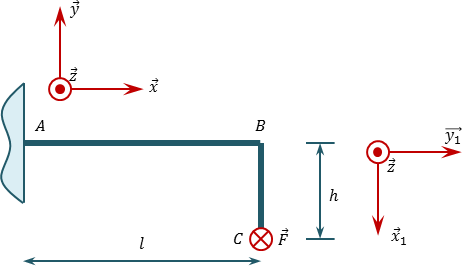
\includegraphics[width=\linewidth]{images/exo_02_corr_01}
\end{center}
\end{minipage}
\end{corrige}
\else 
\fi

\subparagraph{}
\textit{Exprimer le torseur de cohésion dans chacun des tronçons.}

\ifprof
~\\
\begin{corrige} ~\\

\begin{itemize}[label=\ding{112},font=\color{ocre}] 
\item On isole le premier tronçon.
\item Le tronçon est soumis d'une part à l'action mécanique en $A$ (vu qu'on l'a calculée, on va l'utilise ...) et d'autre part à l'action mécanique du torseur de cohésion.
\item On a donc :
\end{itemize}
$$
\torseurscoh_{S-\rightarrow S+} + \torseurcol{0}{0}{-F}{0}{0}{0}{C,\left( \vect{x},\vect{y},\vect{z} \right)} = \{0\}
$$
On a donc :
$$
\torseurscoh_{S+\rightarrow S-}
=\torseurcol{0}{0}{-F}{0}{0}{0}{C,\left( \vect{x},\vect{y},\vect{z} \right)}
$$

$\vectm{G}{\text{Ext}}{\text{Poutre}}
=\vectm{C}{\text{Ext}}{\text{Poutre}} + \vect{GC}\wedge -F \vect{z}  
= \left( (l-x) \vect{x} - h\vect{y} \right) \wedge -F \vect{z}
= F(l-x) \vect{y} +F h\vect{x} 
$
On a donc :
$$
\torseurscoh_{S+\rightarrow S-}
=\torseurcol{0}{0}{-F}{Fh}{F(l-x)}{0}{G,\left( \vect{x},\vect{y},\vect{z} \right)}
$$


\begin{minipage}[c]{.45\linewidth}
\begin{itemize}[label=\ding{112},font=\color{ocre}] 
\item On isole la portion $[GC]$.
\item Le tronçon est soumis d'une part à l'action mécanique en $C$ et d'autre part à l'action mécanique du torseur de cohésion.
\item On a donc :
\end{itemize}
\end{minipage}\hfill
\begin{minipage}[c]{.45\linewidth}
\begin{center}
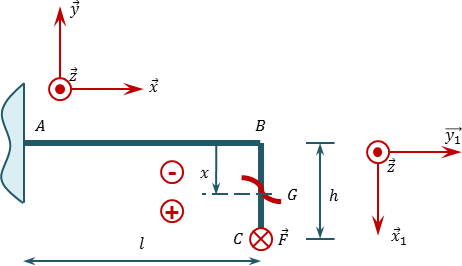
\includegraphics[width=.8\linewidth]{images/exo_02_corr_02}
\end{center}
\end{minipage}
$$
\torseurscoh_{S-\rightarrow S+} + \torseurcol{0}{0}{-F}{0}{0}{0}{C,\left( \vect{x_1},\vect{y_1},\vect{z} \right)} = \{0\}
$$
On a donc :
$$
\torseurscoh_{S+\rightarrow S-}
=\torseurcol{0}{0}{-F}{0}{0}{0}{C}
$$

$\vectm{G}{\text{Ext}}{\text{Poutre}}
=\vectm{C}{\text{Ext}}{\text{Poutre}} + \vect{GC}\wedge -F \vect{z}  
=  (h-x) \vect{x_1}  \wedge -F \vect{z}
=  (h-x) F \vect{y_1}
$. 
On a donc :
$$
\torseurscoh_{S+\rightarrow S-}
=\torseurcol{0}{0}{-F}{0}{(h-x) F}{0}{G,\left( \vect{x_1},\vect{y_1},\vect{z} \right)}
%=\torseurcol{0}{0}{-F}{(h-x) F}{0}{0}{G,\left( \vect{x},\vect{y},\vect{z} \right)}
$$



\end{corrige}
\else 
\fi

\subparagraph{}
\textit{Tracer les diagrammes des sollicitations.}
\ifprof
\begin{corrige}~\\
\begin{center}
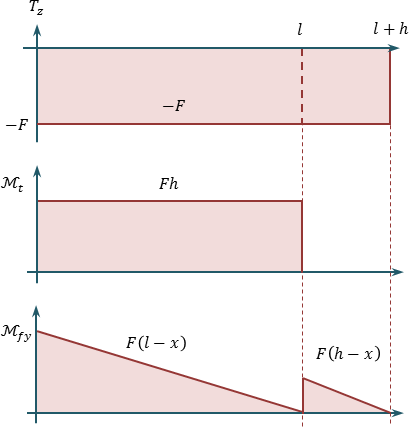
\includegraphics[width=.4\linewidth]{images/exo_02_corr_03}
\end{center}

\end{corrige}
\else 
\fi


\section*{Exercice 4}
\setcounter{subparagraph}{0}
On donne sur le schéma ci-dessous la modélisation d'une poutre et des efforts qui lui sont appliqués.
\begin{center}
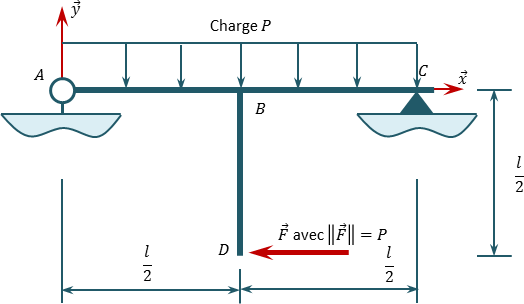
\includegraphics[width=.45\textwidth]{images/exo_03}
\end{center}

\subparagraph{}
\textit{Déterminer les actions mécaniques en $A$ et en $B$.}
\ifprof
\begin{corrige}~\\

Le problème est plan. On isole la poutre et on réalise le bilan des actions mécaniques extérieures (figures ci-dessous). 

\begin{minipage}[c]{.47\linewidth}
On applique le théorème de la résultante statique sur $\vect{x}$ puis sur $\vect{y}$ :
\begin{itemize}[label=\ding{112},font=\color{ocre}] 
\item $X_A-F=0$;
\item $Y_A+Y_C-P=0$.
\end{itemize}
On applique le théorème du moment statique en $A$ en projection sur $\vect{z}$ :
\begin{itemize}[label=\ding{112},font=\color{ocre}] 
\item $-\dfrac{Fl}{2}-\dfrac{Pl}{2}+lY_C=0$.
\end{itemize}
On peut alors résoudre le système : 
$$
\left\{
\begin{array}{l}
X_A=F \\
Y_A=-Y_C+P = 0 \\
Y_C = \dfrac{F+P}{2} = F\\
\end{array}
\right.
$$
\end{minipage}\hfill
\begin{minipage}[c]{.47\linewidth}
\begin{center}
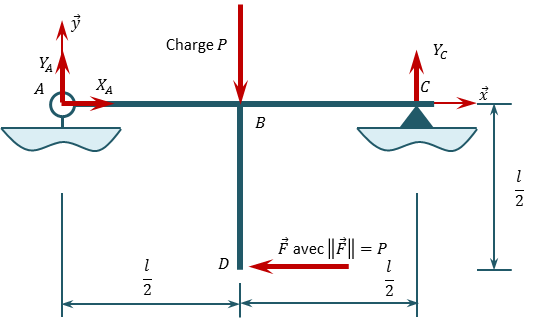
\includegraphics[width=.95\linewidth]{images/exo_03_corr_01}
\end{center}
\end{minipage}
\end{corrige}
\else 
\fi


On cherche à déterminer le diagramme des sollicitations dans chacun des tronçons.

\subparagraph{}
\textit{Quels tronçons peut-on considérer ?}
\ifprof
\begin{corrige}
On peut considérer les tronçons $[AB]$, $[BC]$ et $[BD]$.
\end{corrige}
\else 
\fi

\subparagraph{}
\textit{Exprimer le torseur de cohésion dans chacun des tronçons.}
\ifprof
\begin{corrige}
~\\
\begin{itemize}[label=\ding{112},font=\color{ocre}] 
\item On isole la portion $[AG]$ avec $G \in [AC]$.
\item La portion est soumise d'une part à l'action mécanique en $A$, à l'action uniformément répartie (exprimée en $M$, milieu de $[AG]$) et à l'action mécanique du torseur de cohésion.
\item On a donc : 
\end{itemize}
$$
\torseurscoh_{S+\rightarrow S-} +
 \torseurcol{F}{0}{0}{0}{0}{0}{A,\left( \vect{x},\vect{y},\vect{z} \right)} 
 +\torseurcol{0}{-px}{0}{0}{0}{0}{M,\left( \vect{x},\vect{y},\vect{z} \right)} 
 = \{0\}
$$
On a donc, $\forall x \in \left[0,\dfrac{l}{2}\right]$, 
$$
\torseurscoh_{S+\rightarrow S-}
=-\torseurcol{F}{0}{0}{0}{0}{0}{G}
-\torseurcol{0}{-px}{0}{0}{0}{ \dfrac{px^2}{2}}{G}
=\torseurcol{-F}{px}{0}{0}{0}{-\dfrac{px^2}{2}}{G}
$$
car 
$\vectm{G}{\text{Ext}}{\text{Poutre}}
=\vectm{A}{\text{Ext}}{\text{Poutre}} + \vect{GA}\wedge F \vect{x}  
=  -x\vect{x}  \wedge F \vect{x}
=  \vect{0}
$ 

et 
$\vectm{G}{\text{Ext}}{\text{Poutre}}
=\vectm{M}{\text{Ext}}{\text{Poutre}} + \vect{GM}\wedge \left( -px \right) \vect{y}  
= -\dfrac{x}{2}\vect{x}\wedge \left( -px\right) \vect{y}  
=   \dfrac{px^2}{2} \vect{z}  
$.

\begin{itemize}[label=\ding{112},font=\color{ocre}] 
\item On isole la portion $[GC]$ avec $G\in [BC]$.
\item La portion est soumise d'une part à l'action mécanique en $C$, à l'action uniformément répartie (exprimée en $M$, milieu de $[GC]$) et à l'action mécanique du torseur de cohésion en $G$.
\item On a donc : 
\end{itemize}
$$
\torseurscoh_{S-\rightarrow S+} +
 \torseurcol{0}{F}{0}{0}{0}{0}{C,\left( \vect{x},\vect{y},\vect{z} \right)} 
 +\torseurcol{0}{-p(l-x)}{0}{0}{0}{0}{M,\left( \vect{x},\vect{y},\vect{z} \right)} 
 = \{0\}
$$
On a donc, $\forall x \in \left[\dfrac{l}{2},l\right]$, 
$$
\torseurscoh_{S+\rightarrow S-}
= \torseurcol{0}{F}{0}{0}{0}{(l-x)F}{G} 
 +\torseurcol{0}{-p(l-x)}{0}{0}{0}{-p\dfrac{\left(l-x\right)^2}{2}}{G} 
 = \torseurcol{0}{F-p(l-x)}{0}{0}{0}{(l-x)F-p\dfrac{\left(l-x\right)^2}{2}}{G} 
$$
car 
$\vectm{G}{\text{Ext}}{\text{Poutre}}
=\vectm{C}{\text{Ext}}{\text{Poutre}} + \vect{GC}\wedge F \vect{y}  
=  (l-x)\vect{x}  \wedge F \vect{y}
=  (l-x)F\vect{z}
$ 

et 
$\vectm{G}{\text{Ext}}{\text{Poutre}}
=  \vectm{M}{\text{Ext}}{\text{Poutre}} + \vect{GM}\wedge \left( -p(l-x) \right) \vect{y}  
= \left(\dfrac{l-x}{2}\right)\vect{x}\wedge \left(-p(l-x)\right) \vect{y}  
=  -p\dfrac{\left(l-x\right)^2}{2}\vect{z}  
$.

\begin{center}
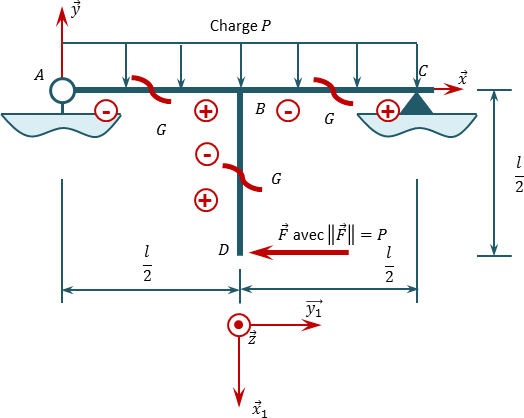
\includegraphics[width=.45\linewidth]{images/exo_03_corr_02}
\end{center}

\begin{itemize}[label=\ding{112},font=\color{ocre}] 
\item On isole la portion $[GD]$ avec $G\in [BD]$.
\item La portion est soumise d'une part à l'action mécanique en $D$ et à l'action mécanique du torseur de cohésion en $G$.
\item On a donc : 
\end{itemize}
$$
\torseurscoh_{S-\rightarrow S+} +
 \torseurcol{0}{-F}{0}{0}{0}{0}{D,\left( \vect{x_1},\vect{y_1},\vect{z_1} \right)} 
 = \{0\}
 \Leftrightarrow
\torseurscoh_{S+\rightarrow S-} =
 \torseurcol{0}{-F}{0}{0}{0}{F \left(x-\dfrac{l}{2}\right) }{G,\left( \vect{x_1},\vect{y_1},\vect{z_1} \right)}  
$$

car
$\vectm{G}{\text{Ext}}{\text{Poutre}}
=  \vectm{D}{\text{Ext}}{\text{Poutre}} + \vect{GD}\wedge \left(-F \right) \vect{y_1}  
= \left(\dfrac{l}{2}-x\right)\vect{x_1}\wedge \left(-F\right) \vect{y_1}  
=F \left(x-\dfrac{l}{2}\right)  \vect{z_1}  
$.


\end{corrige}
\else 
\fi

\subparagraph{}
\textit{Tracer les diagrammes des sollicitations.}
\ifprof
\begin{corrige}~\\

\begin{center}
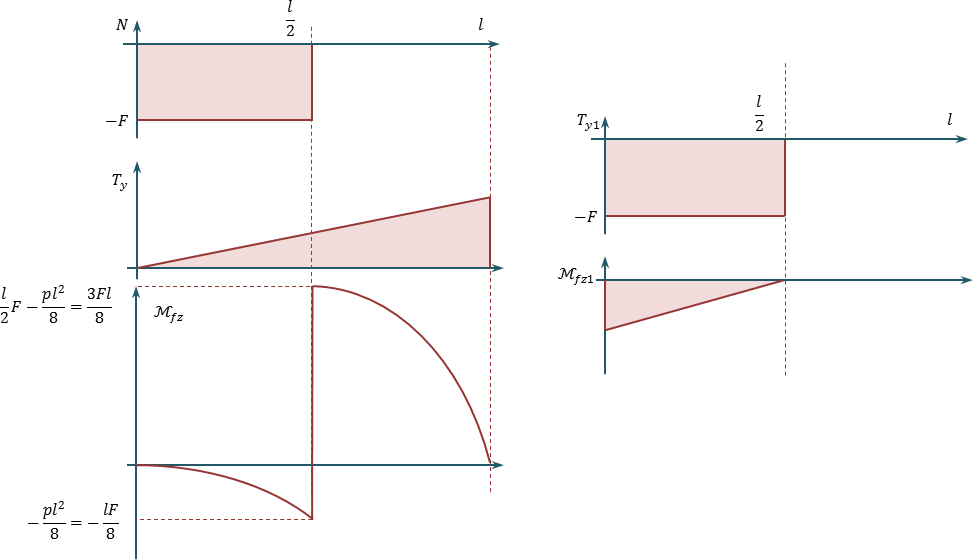
\includegraphics[width=.95\linewidth]{images/exo_03_corr_03}
\end{center}
\end{corrige}
\else 
\fi



\section*{Exercice 7}
\setcounter{subparagraph}{0}
On donne sur le schéma ci-dessous la modélisation d'une poutre et des efforts qui lui sont appliqués.
\begin{center}
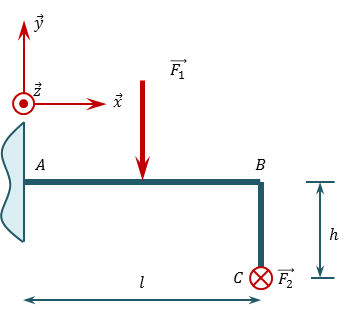
\includegraphics[width=.45\textwidth]{images/exo_07}
\end{center}



On isole la poutre.

La poutre est soumise à l'action mécanique du mur, ainsi qu'aux efforts en $D$ et en $C$ ;
\begin{itemize}
\item $\vect{M(\vect{F_1},A)} 
= \vect{M(\vect{F_1},D)}+\vect{AD}\wedge\vect{F_1}
= \dfrac{l}{2}\vect{x} \wedge F_1 (-\vect{y})
= -\dfrac{l}{2}F_1  \vect{z} $;
\item $\vect{M(\vect{F_2},A)} 
= \vect{M(\vect{F_2},C)}+\vect{AC}\wedge\vect{F_2}
= \left(l\vect{x} - h\vect{y} \right) \wedge\left(-F_2\vect{z}\right)
= F_2l\vect{y} +F_2h\vect{x} $;
\end{itemize}

On applique le PFS au point $A$ et on a : 
\begin{itemize}
\item $X_A=0$;
\item $Y_A - F_1 = 0$;
\item $Z_A - F_2 = 0$;
\item $L_A +F_2h= 0$;
\item $M_A +F_2l=0 $;
\item $N_A -\dfrac{l}{2}F_1=0 $.
\end{itemize}

\textbf{Tronçon $[AC]$}
\begin{itemize}
\item On isole la partie gauche, soumise à l'action mécanique de l'encastrement et à l'action de la partie $+$ sur la partie $-$.
\item On a donc $$
\torseurscoh_{S+\rightarrow S-} +
 \torseurcol{0}{F_1}{F_2}{-F_2h}{-F_2l}{\dfrac{F_1l}{2}}{A} 
 = \{0\} 
 \Leftrightarrow 
 \torseurscoh_{S+\rightarrow S-} 
 =
 -\torseurcol{0}{F_1}{F_2}{-F_2h}{-F_2l}{\dfrac{F_1l}{2}}{A} 
 =
 -\torseurcol{0}{F_1}{F_2}{-F_2h}{-F_2l+\lambda F_2}{\dfrac{F_1l}{2}-\lambda F_1}{G} 
$$
Avec $\vect{M(G)} 
= \vect{M(A)}+\vect{GA}\wedge\left(F_1 \vect{y}+F_2 \vect{z}\right)
= \vect{M(A)}+\left(- \lambda \vect{x}\right)\wedge\left(F_1 \vect{y}+F_2 \vect{z}\right)
= \vect{M(A)}+\left(- \lambda F_1 \vect{z}\right)+\lambda F_2 \vect{y}
$.
\end{itemize}

\textbf{Tronçon $[CB]$}

\begin{itemize}
\item On isole la partie droite, soumise à l'action mécanique de l'effort en $C$ et à l'action de la partie $-$ sur la partie $+$.
\item On a donc $$
\torseurscoh_{S-\rightarrow S+} +
 \torseurcol{0}{0}{-F_2}{0}{0}{0}{C} 
 = \{0\} 
 \Leftrightarrow 
 \torseurscoh_{S+\rightarrow S-} 
 =
 \torseurcol{0}{0}{-F_2}{0}{0}{0}{C} 
 =
  \torseurcol{0}{0}{-F_2}{F_2 h}{F_2 \lambda}{0}{G} 
$$
Avec $\vect{M(G)} 
= \vect{M(C)}+\vect{GC}\wedge\left(-F_2 \vect{z}\right)
= \left(\lambda \vect{x}-h\vect{y} \right)\wedge\left(-F_2 \vect{z}\right)
= F_2\lambda \vect{y}+F_2 h\vect{x} 
$.
\end{itemize}

\textbf{Tronçon $[BC]$}
\begin{itemize}
\item On se positionne dans le repère local $\left(\vect{x_1},\vect{y_1},\vect{z}\right)$.
\item On isole la partie droite, soumise à l'action mécanique de l'effort en $C$ et à l'action de la partie $-$ sur la partie $+$.
\item On a donc $$
\torseurscoh_{S-\rightarrow S+} +
 \torseurcol{0}{0}{-F_2}{0}{0}{0}{C} 
 = \{0\} 
 \Leftrightarrow 
 \torseurscoh_{S+\rightarrow S-} 
 =
 \torseurcol{0}{0}{-F_2}{0}{0}{0}{C,R_1} 
  = \torseurcol{0}{0}{-F_2}{0}{F_2\lambda }{0}{G,R_1}
    = \torseurcol{0}{0}{-F_2}{F_2\lambda}{0 }{0}{G,R}
$$
Avec $\vect{M(G)} 
= \vect{M(C)}+\vect{GC}\wedge\left(-F_2 \vect{z}\right)
= \left(\lambda \vect{x_1} \right)\wedge\left(-F_2 \vect{z}\right)
= F_2\lambda \vect{y_1}
$.
\end{itemize}

\ifprof
\else
\end{multicols}
\fi
\end{document}


